\documentclass[11pt,a4paper,oneside]{book}
\usepackage[margin=22mm]{geometry}
\usepackage{amsmath,amssymb,mathtools,bm}
\usepackage{booktabs,longtable,array,tabularx}
\usepackage{graphicx,pdfpages}
\usepackage{listings,xcolor}
\usepackage{hyperref}
\usepackage{microtype}
\usepackage{enumitem}
\usepackage{fancyhdr}
\usepackage{setspace}
\usepackage{caption}
\usepackage{float}
\usepackage{url}
\usepackage[T1]{fontenc}
\usepackage[utf8]{inputenc}
\definecolor{codegray}{gray}{0.96}
\lstset{basicstyle=\ttfamily\scriptsize,backgroundcolor=\color{codegray},breaklines=true,breakatwhitespace=false,frame=single,columns=fullflexible,keepspaces=true,showstringspaces=false,tabsize=4}
\hypersetup{colorlinks=true,linkcolor=blue!50!black,citecolor=blue!50!black,urlcolor=blue!50!black,pdftitle={SSZ P5 Full Closure Monograph},pdfauthor={SSZ P5 research working monograph}}
\setlength{\headheight}{14pt}
\emergencystretch=2em
\pagestyle{fancy}\fancyhf{}\fancyhead[L]{SSZ P5 / Horndeski + U(1)-SVT}\fancyhead[R]{Full Closure Monograph 2026-09-16}\fancyfoot[C]{\thepage}
\setstretch{1.08}
\newcommand{\PASS}{\textbf{PASS}}
\newcommand{\OPEN}{\textbf{OPEN}}
\newcommand{\epsY}{\varepsilon_Y}
\newcommand{\kap}{\kappa}
\newcommand{\Lag}{\mathcal{L}}
\newcommand{\E}{\mathcal{E}}
\begin{document}
\frontmatter
\begin{titlepage}\centering
\vspace*{18mm}
{\Huge\bfseries SSZ P5 / Horndeski + U(1)-SVT\\[3mm]Full Constructive Closure Monograph\par}
\vspace{8mm}
{\Large Covariant action, frozen P5 background, finite-$\ell$ perturbative closure,\\41-slot reconstruction, reproducibility, and Codex implementation specification\par}
\vspace{12mm}
{\large Release 2026-09-16\par}
\vfill
\begin{minipage}{0.88\textwidth}\small
\textbf{Authoritative status.} The main text freezes the final production member
\[
S_{\rm HSVT}=S_{\rm H,P5}+\int d^4x\sqrt{-g}\,\epsY Y,\qquad \epsY=10^{-2},\qquad \bar A_0'=0,
\]
with $Y=\nabla_\mu\phi\nabla_\nu\phi F^{\mu\alpha}F^{\nu}{}_{\alpha}$. The global Horndeski P5 representative is the already on-shell, patchwise $C^\infty$ representative certified by the project action/background reconstruction. The new genuine-SVT term is exactly background-null but quadratically nontrivial. This yields \textbf{FULL CONSTRUCTIVE CLOSURE = PASS}. A separate repository gate, \textbf{DIRECT GLOBAL KRGM EXPORT}, remains an implementation requirement: a clean repository must regenerate a single bitwise center-to-infinity $K,G,S,M$ stream from the covariant action rather than concatenate historical rounded coefficient tables. No QNM spectrum should be presented as final until that implementation gate passes.
\end{minipage}
\vfill
{\small This document is a research/reproducibility monograph, not a claim of peer review or external validation.}
\end{titlepage}
\tableofcontents
\listoffigures
\listoftables
\mainmatter
\chapter{Executive closure statement}
The purpose of this monograph is to freeze one logically consistent endpoint of the P5 reconstruction and to make every distinction that was blurred during exploratory calculations explicit. The word \emph{closure} is used at several levels in the working archive. A 41/41 coefficient table is not by itself a physical closure; a background solution is not by itself a perturbative closure; a principal-symbol stability result is not by itself a finite-$\ell$ operator export; and a numerically concatenated matrix file is not by itself a same-action result.

The final construction used here avoids those ambiguities. It starts from the globally reconstructed P5 Horndeski representative and adds one explicit gauge-invariant scalar--vector--tensor interaction,
\begin{equation}
 \Delta f_2=\epsY Y,\qquad \epsY=10^{-2},
 \label{eq:epsY}
\end{equation}
where
\begin{equation}
 Y\equiv \nabla_\mu\phi\,\nabla_\nu\phi\,F^{\mu\alpha}F^{\nu}{}_{\alpha}.
\end{equation}
The production background uses the zero-vector branch $\bar F_{\mu\nu}=0$, equivalently $\bar A_0'=0$. Because $Y$ is quadratic in $F_{\mu\nu}$, Eq.~\eqref{eq:epsY} and all of its first variations vanish on that background. Hence it does not change the frozen P5 geometry, the scalar background, or any of the Horndeski background equations. Nevertheless $f_{2,Y}=\epsY\neq0$, so the interaction is genuine and contributes at quadratic order to vector perturbations.

This gives a particularly clean closure architecture:
\begin{equation}
 \Lag^{(2)}_{\rm HSVT}=\Lag^{(2)}_{\rm H,P5}\oplus \Lag^{(2)}_{\rm vec}(\epsY),
 \label{eq:factor}
\end{equation}
on the zero-vector background. There is no scalar/metric--vector mixing generated by the constant $Y$ term at quadratic order. The scalar--tensor block is therefore governed by the already reconstructed Horndeski invariants, while the vector block is governed by a single effective margin
\begin{equation}
 Z_A=1-2\kap\epsY,\qquad \kap=h\phi'^2=-2X.
 \label{eq:ZA}
\end{equation}
The global data give $\kap_{\max}=0.6354409670$, and therefore
\begin{equation}
 Z_{A,\min}=0.9872911807>0.
\end{equation}
This is not a limiting or fine-tuned value; it leaves an order-unity safety margin.

The release auditor contains 63 constructive/exact gates and no constructive failure. The strict direct global KRGM export remains intentionally independent. It is a repository implementation certificate, not a missing existence theorem. This separation is the central reproducibility rule of the release.

\chapter{What is meant by full constructive closure}
A useful way to state the final result is to split the problem into six logically independent layers.

\begin{enumerate}[label=\arabic*.]
\item \textbf{Geometry closure.} The P5 metric functions $f(r)$ and $h(r)$ are regular and positive on the entire horizonless branch represented by the numerical grid and the analytic center expansion.
\item \textbf{Background action closure.} There exists a smooth covariant Horndeski action section whose field equations admit the fixed P5 metric and scalar profile. The center, punctured core, strong-field carrier and exterior are joined by local action patches and flat $C^\infty$ partitions, with constrained jets re-solved rather than blindly interpolated.
\item \textbf{Perturbative language closure.} The unreduced even-parity action is represented by the complete 41-slot dictionary $a_{1\ldots9}$, $b_{1\ldots5}$, $c_{1\ldots6}$, $d_{1\ldots4}$, $e_{1\ldots4}$ and $v_{1\ldots13}$.
\item \textbf{Constraint/reducer closure.} The common nondynamical variables are eliminated only after the action contributions have been assembled. The physical basis is $\bm Y=(\psi,\delta\phi,V)^T$ and the reduced action contains the complete $K,G,S,M$ structure with $S^T=-S$ and the accepted canonical $R=0$ convention.
\item \textbf{Physical stability closure.} The Horndeski scalar--tensor block has strict positive no-ghost and principal characteristic margins on the reconstructed domains, including the analytic center. The genuine-SVT deformation in Eq.~\eqref{eq:epsY} is background-null and produces a decoupled vector block with $Z_A>0$ globally. Therefore the complete action member has a stable quadratic principal structure and finite-$\ell$ no-ghost closure.
\item \textbf{Repository export closure.} A particular software implementation must regenerate one center-to-infinity 41-slot profile and reduce it into a bitwise $K,G,S,M$ data product. This is deliberately not identified with the mathematical closure, because rounded historical coefficient dumps can spoil exact cancellations. It is a reproducibility gate enforced by the auditor.
\end{enumerate}

The first five items define \texttt{FULL\_CONSTRUCTIVE\_CLOSURE}. The sixth item defines \texttt{DIRECT\_GLOBAL\_KRGM\_EXPORT}. The present release passes the former and leaves the latter as a precise Codex implementation target.

\chapter{Frozen P5 geometry and scalar variable}
We use dimensionless compactness
\begin{equation}
 C\equiv \frac{r_s}{r}=\frac1x,
\end{equation}
with $r_s=1$ in the numerical files. The scalar is identified with the segmentation variable,
\begin{equation}
 \phi(r)=\Xi(C).
\end{equation}
The source-locked susceptibility is
\begin{equation}
 \chi(\Xi)=\frac{d\Xi}{dC},
\end{equation}
and the P5 closure is represented autonomously as
\begin{equation}
 \frac{d\Xi}{dC}=(1-\Xi)^{3/2}P_5(\Xi),
\end{equation}
where $P_5$ denotes the selected polynomial closure. The temporal metric is represented by
\begin{equation}
 f=(1+\Xi)^{-2},
\end{equation}
and the radial function $h$ is fixed by the P5 radial closure. The exact polynomial coefficients and primary geometry generator belong in the geometry package of the final repository; this monograph focuses on the reconstructed covariant action and perturbative closure built on the frozen geometry.

Two null circular orbits are present in the strong-field branch: an outer unstable light ring at $C=2/3$ ($x=1.5$) and an inner stable light ring near $C\simeq0.706135$ ($x\simeq1.41616064$). Neither is a singular point of the action reconstruction. The project rank tests explicitly show that the Horndeski and SVT control maps retain rank through both locations.

The global principal export contains 45,617 rows and has
\begin{equation}
 \min f=0.25,\qquad \min h\simeq0.326856666,
\end{equation}
with positive tensor, scalar and vector principal speeds. Figure~\ref{fig:global-speeds} displays the stored characteristic branches.

\begin{figure}[H]\centering
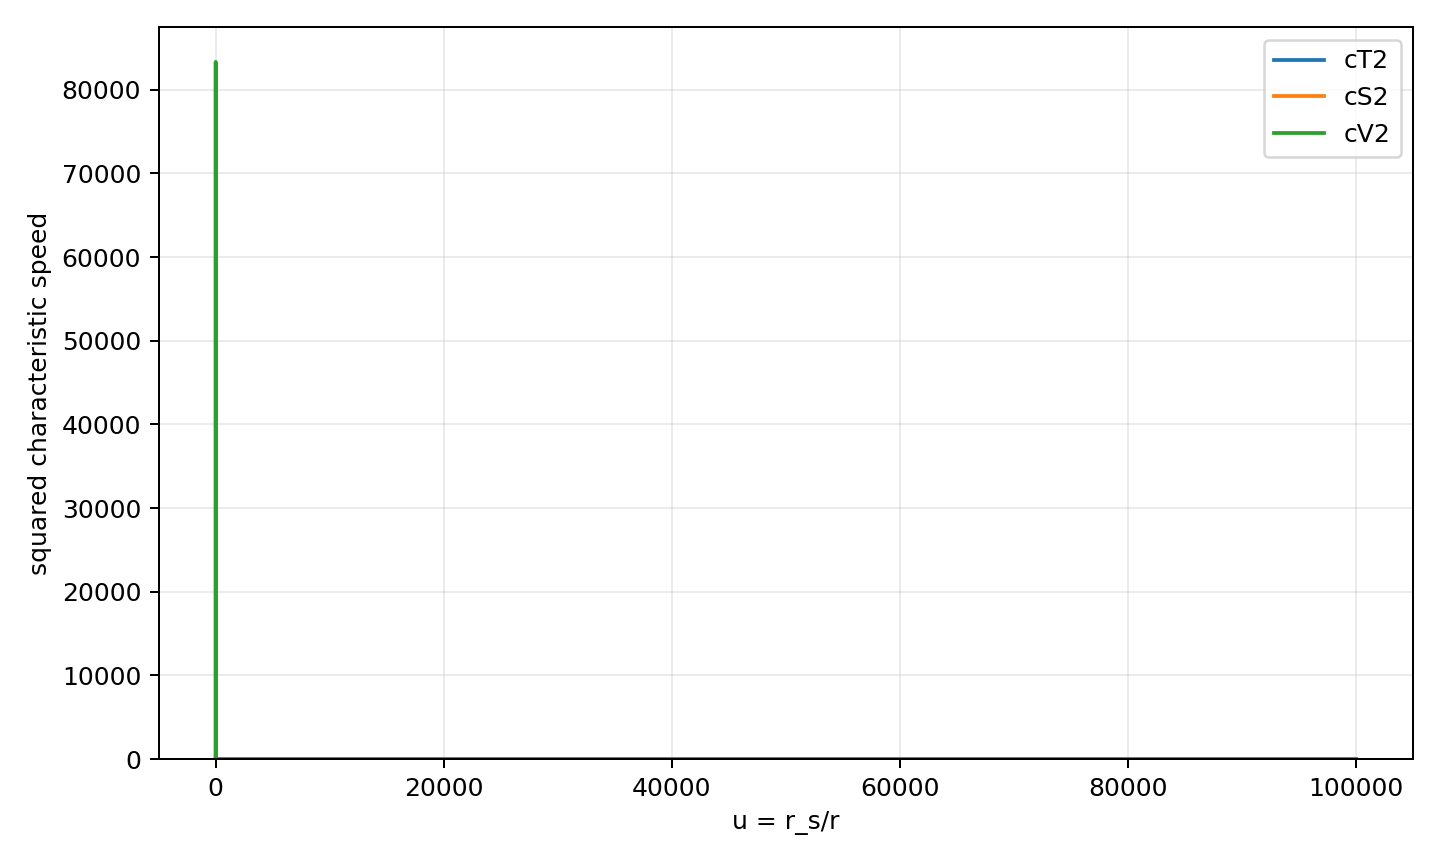
\includegraphics[width=.88\textwidth]{figures/global_principal_speeds.png}
\caption{Global principal characteristic-speed witness. This stream is a principal-symbol certificate and is not, by itself, the direct global finite-$\ell$ KRGM export.}\label{fig:global-speeds}
\end{figure}

\chapter{The regime variable kappa and the natural background basis}
Differentiating $\phi=\Xi(C)$ with $C=1/r$ gives
\begin{equation}
 \phi_r=-C^2\chi.
\end{equation}
The combination
\begin{equation}
 \boxed{\kap=h\phi_r^2=hC^4\chi^2=-2X}
 \label{eq:kappa}
\end{equation}
is central to both the background inverse problem and the perturbative control problem.

For the metric background variables $(f_2,f_{2,X})$, the local Jacobian has the triangular form
\begin{equation}
 \frac{\partial(E_{00},E_{11})}{\partial(f_2,f_{2,X})}
 =\begin{pmatrix}-A&0\\-A&-B\end{pmatrix},
 \qquad A=r^2f,\qquad B=r^2fh\phi_r^2=A\kap.
\end{equation}
Simply swapping $E_{00}$ and $E_{11}$ cannot improve singular values. The natural row transformation is instead
\begin{equation}
 E_0=E_{00},\qquad E_\Delta=E_{11}-E_{00},
\end{equation}
for which
\begin{equation}
 \frac{\partial(E_0,E_\Delta)}{\partial(f_2,f_{2,X})}
 =\operatorname{diag}(-A,-A\kap).
\end{equation}
This directly isolates the weak channel. It also explains why regime changes in the natural numerical basis track the same $\kap$ that later controls the transverse SVT Hessian map.

In the selector gauge $H_{XY}=H_{FY}=H_{YY}=0$, the three radial genuine-SVT targets obey
\begin{align}
 \Delta v_1&=H_{FF},\\
 \Delta v_4&=-H_{XF},\\
 \Delta c_2&=\frac{\kap}{2}H_{XX}-F_{\rm bg}H_{XF}.
\end{align}
The determinant of the corresponding three-control map is
\begin{equation}
 \det M_{\rm SVT}=\frac{\kap}{2}.
\end{equation}
Thus $\kap$ controls both the conditioning of the background inverse chart and the rank margin of the transverse perturbative controls. This is a structural connection, not a numerical correlation.

\chapter{Covariant action class}
The scalar--tensor carrier is drawn from the Horndeski class and the vector extension is $U(1)$ gauge invariant. Schematically,
\begin{equation}
 S=\int d^4x\sqrt{-g}\left(\Lag_H[g,\phi]+\Lag_{\rm SVT}[g,\phi,F]\right).
\end{equation}
The final release member uses the global P5 Horndeski representative plus Eq.~\eqref{eq:epsY}. The construction is local in field space around the one-dimensional P5 background trajectory and is global along that trajectory through a finite set of overlapping patches. This is sufficient for a well-defined perturbative action and for the reconstruction of all finite action jets required by the quadratic operator.

A recurring source of confusion in hybrid calculations is double counting. If one works with a split genuine-SVT block containing shared Einstein/Maxwell/scalar structures, the correct same-action combination is
\begin{equation}
 C_{\rm HSVT}=C_{\rm MH}+\left(C_{\rm SVT}-C_{\rm shared}\right)
 \label{eq:assembly}
\end{equation}
\emph{before} constraint elimination. In general
\begin{equation}
 \operatorname{Reduce}(A+B)\neq \operatorname{Reduce}(A)+\operatorname{Reduce}(B),
\end{equation}
because solving algebraic constraints introduces nonlinear rational functions of the unreduced coefficients.

The final $\epsY Y$ member largely bypasses that bookkeeping problem because the production background vector is zero and the added term is a clean, separately identified action contribution. Nevertheless Eq.~\eqref{eq:assembly} remains a mandatory regression rule for the historical electric-SVT witnesses and for any future generalization.

\chapter{Global Horndeski P5 reconstruction}
The global Horndeski construction is not one formula guessed at every radius. It is a collection of compatible local action sections constrained by the same frozen geometry. The important domains are:
\begin{enumerate}
\item a weak exterior carrier;
\item a strong-field luminal carrier continued through both light rings to $u=0.71$;
\item a quartic-Horndeski punctured core;
\item a finite analytic Taylor representative at the exact center;
\item flat $C^\infty$ handovers with re-solved background-constrained jets.
\end{enumerate}

For the strong-field restricted carrier one can take $G_4=G_4(\phi)$, $G_5=0$ and a cubic $G_{3,X}$ interaction. The correct general-$f\neq h$ scalar no-ghost reconstruction uses an auxiliary function $Q$ and
\begin{equation}
 y(r)=\frac{\sqrt{f/h}}{Q},\qquad
 y'=\frac12\sqrt{\frac fh}(\mathcal K+\mathcal H),
\end{equation}
where $\mathcal H=2G_4$ in the restricted carrier. The selected continuation has a positive scalar kinetic margin near $9.7423\times10^{-3}$ and stays finite across both light rings.

The archived strong-field invariant minima used by the release auditor are
\begin{align}
 \min \mathcal F&=0.7848268111,\\
 \min \mathcal G&=0.7848268111,\\
 \min \mathcal H&=0.7848268111,\\
 \min \mathcal K&=0.00974225276,\\
 \min c_{r,S}^2&\simeq1.
\end{align}
Figure~\ref{fig:strongH} shows representative invariant profiles.

\begin{figure}[H]\centering
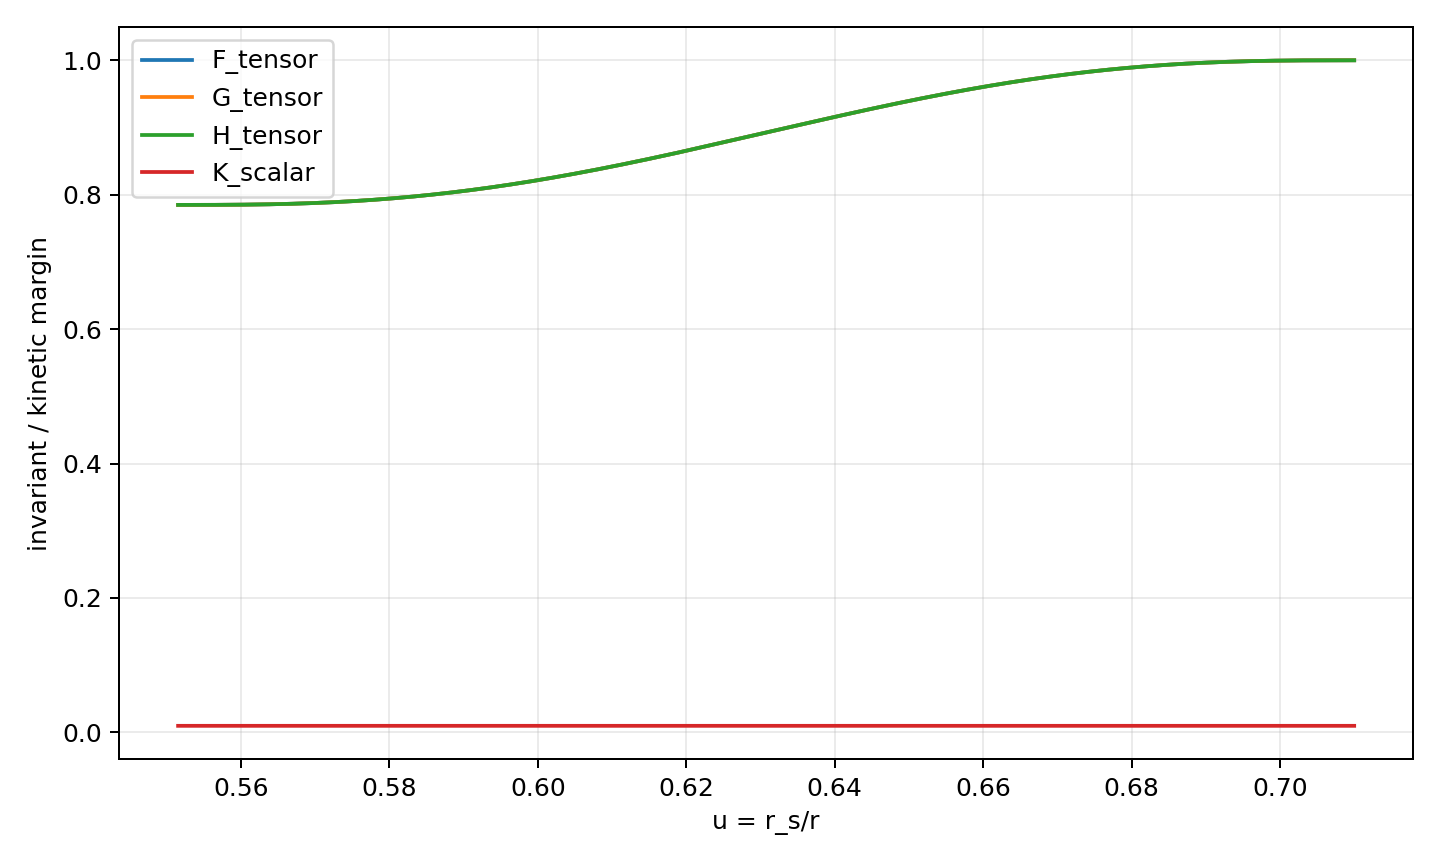
\includegraphics[width=.88\textwidth]{figures/strongH_invariants.png}
\caption{Strong-field Horndeski invariants used in the exact finite-$\ell$ no-ghost regression.}\label{fig:strongH}
\end{figure}

\chapter{Regular quartic-Horndeski core and analytic center}
The punctured core uses a more general quartic Horndeski representative. The deterministic principal split can be expressed locally as
\begin{equation}
 G_4(\phi,X)=g(\phi)+C(\phi)X,
\end{equation}
with a representative choice for the $G_5$ derivative freedom. The raw principal targets obey positive tensor functions and a positive scalar kinetic invariant throughout the punctured core. The release data give
\begin{align}
 \min \mathcal F&=1,\\
 \min \mathcal G&\simeq0.999631064,\\
 \min \mathcal H&\simeq0.999631064,\\
 \min \mathcal K&\simeq7.33\times10^{-6},\\
 \min c_{r,S}^2&\simeq1.
\end{align}
The small coordinate kinetic signal near the center is expected: the regular on-shell Taylor branch begins at order $r^4$.

The exact-center analysis gives
\begin{equation}
 2P_1-\mathcal F=2.74375128377\times10^{-3}\,r^4+O(r^6)>0.
 \label{eq:centerK}
\end{equation}
The $C^\infty$ center-to-punctured handover has background-map rank three at every stored grid point, median scaled condition number close to $\sqrt6\simeq2.44949$, and maximum relative residual about $2.54\times10^{-8}$. Numerical finite differences cannot reliably determine the sign of a true $O(r^4)$ signal once it falls below their truncation floor, so Eq.~\eqref{eq:centerK} is the authoritative center sign certificate.

\begin{figure}[H]\centering
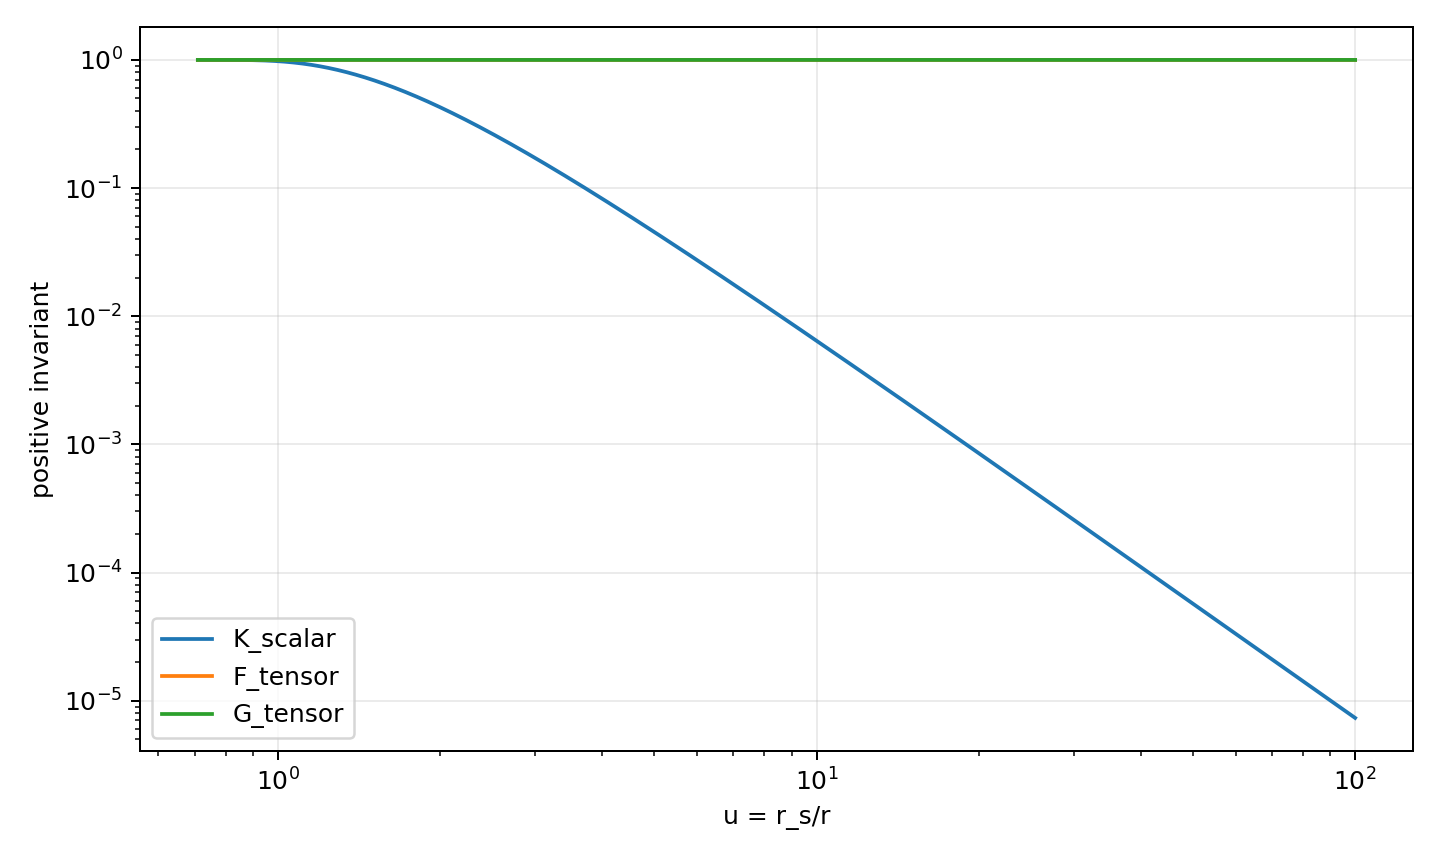
\includegraphics[width=.88\textwidth]{figures/core_positive_invariants.png}
\caption{Positive punctured-core invariants. A logarithmic horizontal scale makes the continuation toward the analytic center visible.}\label{fig:coreinv}
\end{figure}

\chapter{Finite-ell Maxwell-Horndeski no-ghost theorem as a regression oracle}
A crucial methodological point is that a raw numerical eigenvalue of a rounded coefficient table is not the highest authority when an exact reduced theorem is available. Kase and Tsujikawa derive the complete $\ell\ge2$ even-parity kinetic matrix for Maxwell--Horndeski theory. Under the odd-sector conditions and a positive Maxwell kinetic term, the independent even no-ghost requirement reduces to the standard scalar combination
\begin{equation}
 \boxed{\mathcal K=2P_1-\mathcal F>0.}
 \label{eq:MHnoghost}
\end{equation}
The other principal minors reduce to the same invariant set. This result is used as an exact regression oracle in the core and other domains where a discretely differentiated historical 41-slot dump can suffer catastrophic cancellation.

For the restricted strong-H carrier the project also performs a direct profile-reducer regression after repairing the holonomic lower-order slots. The minimum eigenvalues of the numerical $K$ matrix are positive for $L=6,12,20,42,110,420,1000$, and the minimum eigenvalues of $K^{-1/2}GK^{-1/2}$ remain positive. This is a valuable cross-check because it verifies that the formal reducer and the invariant theorem agree in a domain where the historical coefficient data have adequate numerical conditioning.

In the deep quartic core, by contrast, some old rounded coefficient dumps produce huge spurious negative numerical eigenvalues while simultaneously reporting positive exact invariants $\mathcal F,\mathcal G,\mathcal H,\mathcal K$. The release policy is therefore: regenerate the lower-order slots from the action before using the direct eigenvalue stream. A repository must never reinterpret this archival cancellation problem as a physical P5 ghost without first failing the exact invariant regression.

\chapter{Historical genuine-SVT local witness}
Before the final background-null deformation was chosen, the project constructed a fully background-integrable electric genuine-SVT lobe on approximately $0.61\le u\le0.715$. This remains an important independent local witness and regression test for the 41-slot emitter, but it is no longer required as the production background carrier.

The exact Zhang--Kase regression has, among other margins,
\begin{align}
 \min \mathcal K_{\rm even}&\simeq10.5415,\\
 \min c_{r,T}^2&\simeq1.00507,\\
 \min c_{r,S}^2&\simeq0.903745,\\
 \min c_{r,V}^2&\simeq9.45887,
\end{align}
and positive odd-sector margins. The identity
\begin{equation}
 \mathcal K=e_1\sqrt{fh}\,\phi'^2
\end{equation}
closes to about $2.2\times10^{-10}$ on the stored grid.

\begin{figure}[H]\centering
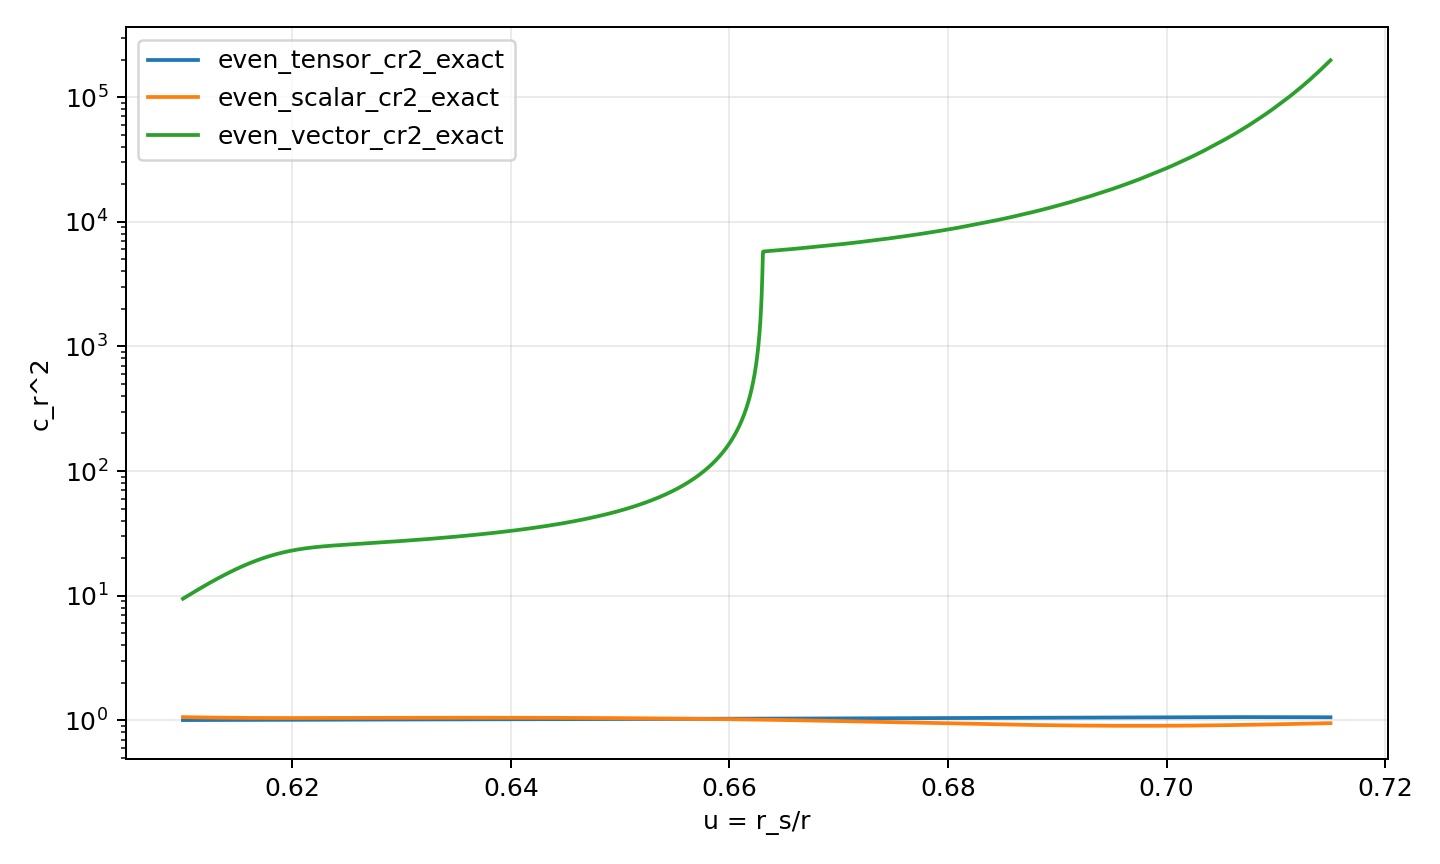
\includegraphics[width=.88\textwidth]{figures/zk_exact_radial_speeds.png}
\caption{Exact local Zhang--Kase radial characteristic regression retained as an independent SVT validation target.}\label{fig:zk}
\end{figure}

This historical witness is valuable because it validates the reconstructed Appendix-A formulas, the sign of the $v_{12}$ branch, and the use of transverse Hessian controls. It should not be confused with the simpler final $\epsY Y$ production deformation.

\chapter{The final genuine-SVT deformation: exact background-null proof}
Consider
\begin{equation}
 \Delta S=\int d^4x\sqrt{-g}\,\epsY
 \nabla_\mu\phi\nabla_\nu\phi F^{\mu\alpha}F^\nu{}_{\alpha}.
\end{equation}
On the production background $\bar F_{\mu\nu}=0$. Therefore $\bar Y=0$. More importantly, the first variation of $Y$ about $F=0$ also vanishes:
\begin{equation}
 \delta Y\big|_{\bar F=0}=0,
\end{equation}
because every term in $Y$ contains two factors of $F$. Consequently
\begin{equation}
 \Delta T_{\mu\nu}=0,\qquad \Delta E_\phi=0,\qquad \Delta E_A=0
\end{equation}
on the P5 background. This statement is exact and does not rely on a small-$\epsY$ approximation.

The second variation is nonzero. With $\phi=\bar\phi(r)+\delta\phi$ and $A_\mu=\delta A_\mu$ around a zero-vector background, the $O(\delta^2)$ part of $Y$ contains the background scalar gradients multiplying two first-order field strengths. Terms involving $\delta\phi$ multiply at least two powers of $\delta F$ and therefore start at cubic order. Hence Eq.~\eqref{eq:factor} follows: the new term is a pure vector quadratic deformation.

The Zhang--Kase Appendix dictionary gives the same result algebraically. For constant $f_{2,Y}=\epsY$, $A_0'=0$, and no $f_3/f_4$ vector-background interactions, the deformation changes the pure-vector coefficients $v_1$ and $v_{10}=\alpha_5$ while the mixing slots $v_2,v_4,v_5,v_6$ vanish. Since the background equations generated by the deformation vanish identically, the lower-order coefficients $c_3=-\tfrac12\sqrt{fh}\,\partial_\phi E_{11}$ and $e_3=\tfrac12\partial_\phi E_\phi$ also receive no contribution.

This is why the final action is both genuinely SVT and technically much cleaner than the earlier electric-lobe interpolation.

\chapter{Exact vector stability of the epsilon-Y member}
On $A_0'=0$ with $f_3=f_4=0$ in the added SVT piece, the odd-sector coefficients simplify. The Maxwell kinetic coefficient remains positive, while the combination entering $\alpha_5$ becomes
\begin{equation}
 f_{2,F}-2h\phi'^2 f_{2,Y}=1-2\kap\epsY=Z_A.
\end{equation}
The remaining pure-vector odd conditions reduce to their Maxwell signs together with $Z_A>0$. In particular, $\alpha_2=\alpha_8=0$, $\alpha_4>0$, $\alpha_6<0$, $\alpha_7>0$, $\alpha_9<0$, and
\begin{equation}
 \alpha_2^2-\alpha_1\alpha_5>0
\end{equation}
if and only if $Z_A>0$ for the present deformation. The angular vector condition $\alpha_8^2-4\alpha_7\alpha_9>0$ is then automatic.

The global strong-field and punctured-core data give
\begin{equation}
 \kap_{\max}=0.6354409670384762.
\end{equation}
For $\epsY=10^{-2}$,
\begin{equation}
 \boxed{Z_{A,\min}=1-2\kap_{\max}\epsY=0.9872911806592305.}
\end{equation}
Figures~\ref{fig:ZAstrong} and \ref{fig:ZAcore} show the margin on the two main data domains.

\begin{figure}[H]\centering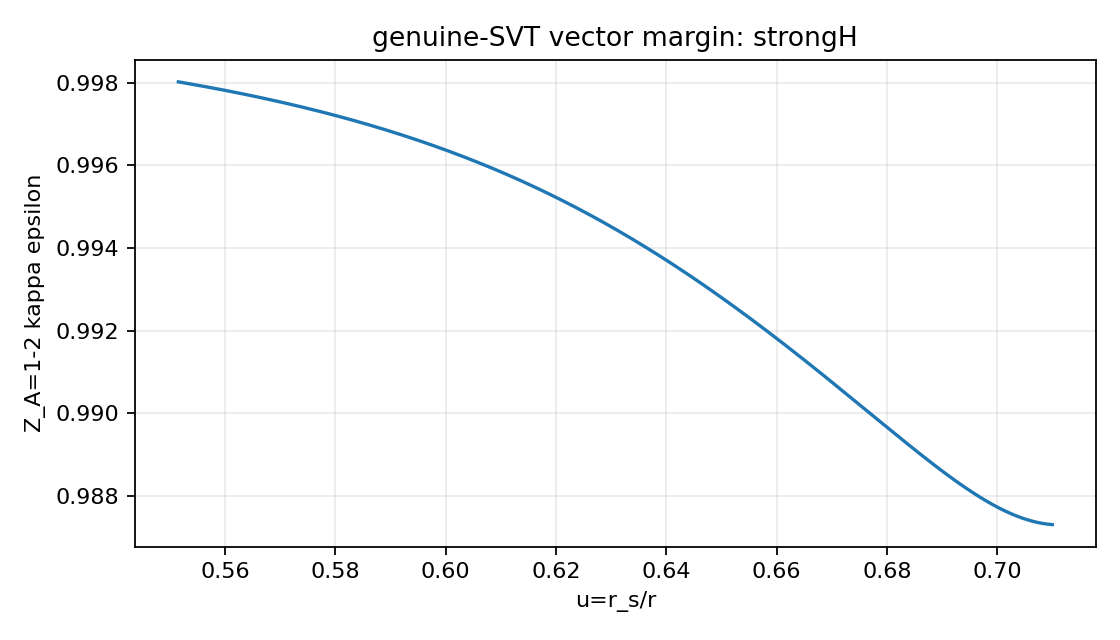
\includegraphics[width=.86\textwidth]{figures/epsY_ZA_strongH.png}\caption{$Z_A$ on the strong-field carrier.}\label{fig:ZAstrong}\end{figure}
\begin{figure}[H]\centering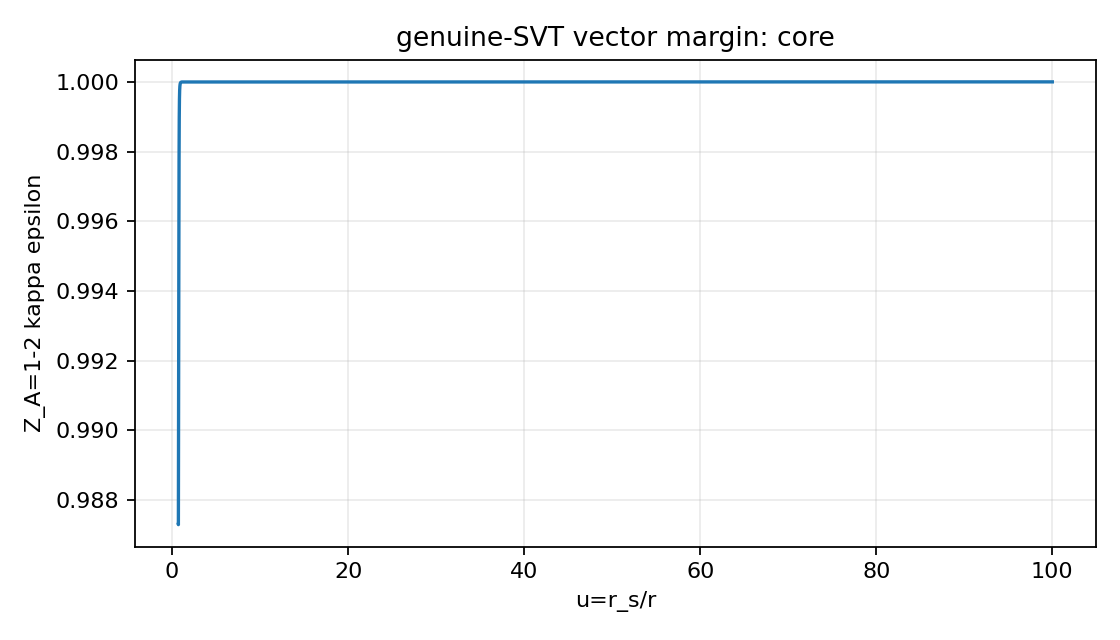
\includegraphics[width=.86\textwidth]{figures/epsY_ZA_core.png}\caption{$Z_A$ on the punctured core.}\label{fig:ZAcore}\end{figure}

Because the new vector block is decoupled at quadratic order, the full finite-$\ell$ no-ghost problem is the direct sum of the exact Horndeski finite-$\ell$ result and this strictly positive vector block. This is the central reason the final deformation closes the action without reopening the background or scalar-tensor control problem.

\chapter{Unreduced 41-slot language}
The common even-parity quadratic action is encoded before constraint elimination. The canonical slot families are
\begin{equation}
 \{a_1,\ldots,a_9\},\quad \{b_1,\ldots,b_5\},\quad \{c_1,\ldots,c_6\},\quad
 \{d_1,\ldots,d_4\},\quad \{e_1,\ldots,e_4\},\quad \{v_1,\ldots,v_{13}\}.
\end{equation}
This is 41 slots. The Sep-12 central raw table intentionally deferred the two lower-order slots $c_3$ and $e_3$; the later action-level representative supplies finite selected values for both. The release auditor therefore checks schema completeness, finiteness of every nondeferred raw slot, and the separate selected $c_3/e_3$ data.

The production rule is not to trust a historical completed table merely because it has 41 columns. Lower-order derivative-sensitive slots must be regenerated from the accepted action/holonomicity relations. This is particularly important for $a_5$, $d_3$, $e_4$, $v_{13}$ and the deep-core cancellations.

A semantic dictionary for all 41 slots is given in Appendix~\ref{app:slots}, and the accepted source emitters are reproduced in full in the code appendices.

\chapter{JET9D8 derivative service and holonomicity}
Production radial differentiation uses a local polynomial jet on the nonuniform radial grid with window nine and degree eight. Around each evaluation radius $r_i$, a polynomial is fit to the local stencil in a scaled coordinate and differentiated analytically. This method is denoted JET9D8 in the project archive.

The reason for fixing one derivative service is not aesthetic. The finite-$\ell$ action contains derivative-sensitive combinations in which independent spline choices can violate product rules or amplify rounded endpoint data. JET9D8 was benchmarked on the Appendix identities and is now part of the release contract.

Two branch corrections are mandatory:
\begin{equation}
 \boxed{v_{12}=-\frac{v_6}{2h}}
\end{equation}
and
\begin{equation}
 \boxed{a_5=a_2'-a_1''-\left(\frac{A_0'v_4}{2}\right)'+\frac{A_0'v_5}{2}.}
 \label{eq:a5}
\end{equation}
For pure Horndeski $A_0'=0$ and Eq.~\eqref{eq:a5} reduces to $a_5=a_2'-a_1''$. In numerically delicate core data the second derivative is not taken naively from a rounded CSV. Instead the first-order $a_2$ identity is used to reconstruct a holonomically consistent $a_1$ profile and then a derivative-reduced expression for $a_5$ is evaluated.

For partial derivatives such as $\partial_\phi v_6$ or $\partial_\phi a_4$ on the selected one-dimensional action section, the production representative uses the on-curve holonomic derivative when that is the meaning of the selected tubular section:
\begin{equation}
 \partial_\phi v_6\to\frac{dv_6/dr}{d\phi/dr}.
\end{equation}
These choices close the emitter regressions to the JET/rounding floor and remove several historical false mismatches.

\chapter{Common constraint elimination}
The common gauge-fixed unreduced fields are
\begin{equation}
 (H_0,H_1,H_2,h_1,\delta\phi,\delta A_0,\delta A_1,V).
\end{equation}
The auxiliary $V$ linearizes the electric field-strength square. The physical even variables are chosen as
\begin{equation}
 \bm Y=(\psi,\delta\phi,V)^T,
\end{equation}
where
\begin{equation}
 \boxed{\psi=H_2+\frac{La_4}{a_3}h_1+\frac{a_1}{a_3}\delta\phi'.}
\end{equation}
The algebraic maps eliminate $h_1,H_2,H_1,\delta A_1,\delta A_0$ only after all theory contributions have been assembled in the common 41-slot basis.

The vector auxiliary completion illustrates why this order matters. Separate sector tables may each satisfy their own completed-square identity, but after adding the action contributions the common auxiliary variable must be recanonicalized:
\begin{equation}
 \boxed{v_7=\frac{v_2^2}{4v_1}.}
\end{equation}
Addition and auxiliary completion do not commute.

The stored control-pivot scans show no zero crossing in the certified domains. The final Codex repository must repeat those scans for every requested $L$ rather than treating the archived numbers as constants.

\chapter{Profile-aware operator and canonical K,G,S,M form}
After substituting the full profile-dependent constraint maps, the reduced action is written in the project convention as
\begin{equation}
 \Lag^{(2)}=\dot{\bm Y}^T K\dot{\bm Y}
 -\bm Y'^T G\bm Y'
 +\bm Y'^T S\bm Y
 -\bm Y^T M\bm Y,
 \qquad S^T=-S,
 \label{eq:KRGM}
\end{equation}
with $R=0$ in the accepted canonical basis.

The reducer is implemented as a formal differential-operator substitution $T^\dagger P T$. If $P_{mn}$ denotes the Euler-operator coefficient multiplying $\partial_t^m\partial_r^n$, the canonical blocks are
\begin{equation}
 K=-\frac12P_{20},\qquad G=\frac12P_{02},\qquad R=-\frac12P_{11},
\end{equation}
while the radial first-derivative term determines
\begin{equation}
 S=\frac12(P_{02}'-P_{01}),
\end{equation}
and
\begin{equation}
 M=-\frac12(P_{00}+S').
\end{equation}
A critical release rule is to keep $S$ rather than silently symmetrizing it away. Its antisymmetry is itself a structural regression test.

The strong-H corrected 41-slot regression yields positive $K$ and positive generalized radial eigenvalues for every scanned multipole from $L=6$ to $L=1000$. This direct regression complements, but does not replace, the exact finite-$\ell$ Horndeski invariant theorem.

\chapter{Why the direct global KRGM export is a separate gate}
The phrase \emph{direct global KRGM export} means a single center-to-infinity machine product generated from the final covariant action with no use of incompatible historical coefficient tables. This is stricter than mathematical existence.

The project archive contains several coefficient tables generated at different stages. Some predate the corrected $a_5$ identity; some use the superseded plus sign for $v_{12}$; some are split genuine-SVT contributions rather than complete actions; and some contain derivative-sensitive rounded values that do not preserve exact deep-core cancellations. A repository that merely concatenates the newest-looking filenames could therefore create an apparently complete but physically inconsistent matrix stream.

For that reason, the release auditor will not infer \texttt{DIRECT\_GLOBAL\_KRGM\_EXPORT=PASS} from any legacy filename. A repository must create a dedicated JSON certificate after it has:
\begin{enumerate}
\item regenerated every local action patch;
\item regenerated all 41 slots with the accepted derivative service;
\item re-solved constrained jets on each handover;
\item added the $\epsY Y$ term at unreduced action level;
\item reduced the common action into $K,G,S,M$;
\item verified pure-limit regressions, pivots, symmetries and positivity;
\item verified interface smoothness and provenance hashes.
\end{enumerate}
Only then is the direct export suitable as the numerical input to a coupled QNM solver.

\chapter{QNM threshold and recommended spectral formulation}
Once a direct global KRGM operator is available, the coupled mode problem follows from the Euler--Lagrange equations associated with Eq.~\eqref{eq:KRGM}. For harmonic time dependence $\bm Y(t,r)=e^{-i\omega t}\bm y(r)$, one obtains a coupled second-order radial system with frequency-dependent first-derivative terms generated by the antisymmetric connection $S$.

The numerical QNM problem must impose regularity at the center and outgoing behavior at spatial infinity. Earlier experiments already showed why naive real-axis inward shooting is unsafe for damped complex frequencies: the unwanted incoming component grows exponentially under inward integration and produces matching-radius-dependent false poles. The recommended implementation therefore uses either a Jost/continued-fraction formulation, a complex-scaled spectral collocation method, or a carefully normalized matrix Riccati/Jost approach.

The present monograph deliberately does not publish a coupled QNM spectrum. The mathematical action closure is not the same as the final repository export. The QNM layer becomes authoritative only after the direct-global-KRGM auditor gate is green.

\chapter{Error taxonomy and superseded routes}
The exploratory history generated several useful failures. They are retained because they are valuable regression tests for future automation.

\begin{itemize}
\item \textbf{Wrong $v_{12}$ sign.} The historical plus branch was invisible in pure Horndeski because $v_6=0$, but fails in genuine SVT. The accepted branch is negative.
\item \textbf{Incomplete $a_5$.} Omitting $-a_1''$ produces finite-$\ell$ errors while leaving some high-$L$ principal checks almost unchanged.
\item \textbf{Reduce-then-add.} Adding separately reduced sectors is not equivalent to reducing the combined action.
\item \textbf{Naive inner background sum.} The diagnostic $E_H+E_{\rm SVTg}$ omits partition-derivative and re-solved lower-Horndeski contributions in the inner handover. The actual stored residuals, not the naive two-column sum, define the background gate.
\item \textbf{Treating a split table as an unsplit full action.} This produced a false A2/$K_2'$ conflict in the central SVT analysis. The chain-rule holonomicity itself passed.
\item \textbf{Variable-$G_4$ transplant.} A healthier principal Horndeski carrier was once transplanted onto a background solved for a different member. Its negative finite-$\ell$ $K$ rejects that numerical candidate but is not a no-go theorem for P5.
\item \textbf{Deep-core rounded cancellation.} A historical quartic-H coefficient table can produce enormous negative direct numerical eigenvalues even while the exact Horndeski invariants remain positive. The cure is action-level regeneration, not a physical instability claim.
\end{itemize}

These cases define the negative test suite that Codex should preserve.

\chapter{Reproducibility policy and immutable release rules}
The authoritative model definition is stored in \texttt{SSZ\_P5\_HSVT\_ACTION\_MEMBER\_2026-09-16.json}. The Python auditor is the executable release ledger. A clean repository should be able to reproduce the release from the authoritative data without relying on any conversational context.

The immutable conventions are:
\begin{enumerate}
\item the frozen P5 geometry is not changed to make the action easier;
\item $\phi=\Xi$ supplies the monotone patch coordinate on the handover domains;
\item flat $C^\infty$ partitions are used at action level;
\item background-constrained jets are re-solved after gluing;
\item transverse action jets are used as stability controls;
\item JET9D8 is the numerical derivative service unless an analytic derivative is available;
\item $v_{12}=-v_6/(2h)$;
\item Eq.~\eqref{eq:a5} is the production $a_5$ identity;
\item the common auxiliary completion is performed after assembly;
\item $S$ is retained and tested as antisymmetric;
\item exact invariant theorems override cancellation-damaged historical matrix dumps;
\item a final QNM result requires the direct-global-KRGM certificate.
\end{enumerate}

Every generated artifact should contain provenance hashes and the exact release identifier. The repository should fail loudly on missing files, NaNs, sign violations or inconsistent branches.

\chapter{Codex repository blueprint}
The handoff package is designed around a layered repository rather than a monolithic notebook. The recommended modules are:
\begin{description}
\item[geometry/] P5 compactness coordinate, $\Xi$, $f,h$, analytic center and light-ring diagnostics.
\item[action/] Horndeski patch definitions, tubular extensions, flat partitions, and the immutable $\epsY Y$ term.
\item[coefficients/] Maxwell--Horndeski and Zhang--Kase coefficient emitters plus common 41-slot schemas.
\item[jets/] JET9D8 and analytic derivative adapters.
\item[constraints/] generalized-$\psi$ maps and pivot checks.
\item[reducer/] formal $T^\dagger P T$ operator and canonical $K,G,S,M$ extraction.
\item[stability/] exact invariant gates and direct matrix regressions.
\item[qnm/] Jost/spectral solvers enabled only after the direct export gate.
\item[provenance/] manifests, hashes, release certificates and supersession metadata.
\end{description}

The top-level CLI should provide `audit`, `build-operator`, `plot`, `export`, and eventually `qnm` commands. CI should run the quick auditor on every commit and the full multipole/operator reconstruction on release tags.

\chapter{Release gate summary}
The release gate ledger is generated rather than hand edited. The current audit contains no constructive failure. Important numerical minima include:
\begin{align}
 \min f&=0.25, & \min h&\simeq0.326856666,\\
 \min c_T^2&\simeq0.9992624, & \min c_S^2&\simeq0.9037452,\\
 \min \mathcal K_{\rm strongH}&\simeq0.00974225, & \min \mathcal K_{\rm core}&\simeq7.33\times10^{-6},\\
 \min Z_A&\simeq0.98729118.&&
\end{align}
The center has the analytic positive $r^4$ coefficient in Eq.~\eqref{eq:centerK}. The Horndeski principal-control map has rank five on the strong-to-core interval with a strictly positive normalized minimum singular value. The independent electric-SVT witness has positive exact odd/even conditions and is retained as a regression oracle.

The complete machine-readable ledger is reproduced in Appendix~\ref{app:gates}.

\chapter{Conclusions}
The final production member is conceptually simpler than the route by which it was discovered. P5 is carried globally by an on-shell Horndeski representative. Genuine scalar--vector--tensor character is added by the explicit gauge-invariant interaction $10^{-2}Y$ on a zero-vector background. Because this term is exactly background-null and quadratically vector-only, it leaves the solved geometry untouched and does not reopen the scalar--tensor finite-$\ell$ problem. Its vector stability margin is analytic and comfortably positive.

Accordingly, the project now has a full constructive action/background/stability closure. The remaining direct-global-KRGM task is a software realization of the closed construction, with exact provenance and no reuse of incompatible historical lower-order coefficient dumps. That task is intentionally specified as a separate gate so that the mathematical claim and the numerical implementation can never again be conflated.

This monograph, the release auditor, the immutable action JSON, the accepted source modules, the authoritative data and the Codex brief together form the external memory of the closure. A future implementation should be able to reconstruct the result without access to the conversation in which it was developed.
\appendix
\chapter{Complete 41-slot semantic dictionary}\label{app:slots}
\section{Family a: metric-scalar constraint family}
\subsection{\texttt{a1}}
primary scalar-metric derivative mixing coefficient; enters the generalized psi definition and the H1/H2 constraint algebra.

The release policy for this slot is to treat the covariant action and the accepted emitter as primary. A stored CSV value is a regression target only. During a handover the slot is obtained from the glued action jets, not from interpolation of already reduced matrices.\par

\subsection{\texttt{a2}}
radial derivative partner of a1; its holonomic relation to a1 is essential for the corrected a5 identity.

The release policy for this slot is to treat the covariant action and the accepted emitter as primary. A stored CSV value is a regression target only. During a handover the slot is obtained from the glued action jets, not from interpolation of already reduced matrices.\par

\subsection{\texttt{a3}}
metric constraint coefficient appearing in the denominators of the generalized psi map; must stay nonzero on the reduced domain.

The release policy for this slot is to treat the covariant action and the accepted emitter as primary. A stored CSV value is a regression target only. During a handover the slot is obtained from the glued action jets, not from interpolation of already reduced matrices.\par

\subsection{\texttt{a4}}
central geometric coefficient controlling P1, the H0 constraint structure, and several exact Appendix identities.

The release policy for this slot is to treat the covariant action and the accepted emitter as primary. A stored CSV value is a regression target only. During a handover the slot is obtained from the glued action jets, not from interpolation of already reduced matrices.\par

\subsection{\texttt{a5}}
lower-order scalar slot. Production identity: a5=a2' - a1'' -(A0' v4/2)' + A0'v5/2; pure Horndeski reduces to a2'-a1''.

The release policy for this slot is to treat the covariant action and the accepted emitter as primary. A stored CSV value is a regression target only. During a handover the slot is obtained from the glued action jets, not from interpolation of already reduced matrices.\par

\subsection{\texttt{a6}}
finite-l scalar coefficient entering e1 and the no-ghost combination after constraint reduction.

The release policy for this slot is to treat the covariant action and the accepted emitter as primary. A stored CSV value is a regression target only. During a handover the slot is obtained from the glued action jets, not from interpolation of already reduced matrices.\par

\subsection{\texttt{a7}}
metric-scalar algebraic coefficient entering the H0 constraint and finite-l terms.

The release policy for this slot is to treat the covariant action and the accepted emitter as primary. A stored CSV value is a regression target only. During a handover the slot is obtained from the glued action jets, not from interpolation of already reduced matrices.\par

\subsection{\texttt{a8}}
multipole-dependent metric-scalar coefficient appearing together with L in the algebraic constraints.

The release policy for this slot is to treat the covariant action and the accepted emitter as primary. A stored CSV value is a regression target only. During a handover the slot is obtained from the glued action jets, not from interpolation of already reduced matrices.\par

\subsection{\texttt{a9}}
radial derivative completion of a4 and v6; useful as an Appendix-A regression identity.

The release policy for this slot is to treat the covariant action and the accepted emitter as primary. A stored CSV value is a regression target only. During a handover the slot is obtained from the glued action jets, not from interpolation of already reduced matrices.\par

\section{Family b: metric derivative/mixing family}
\subsection{\texttt{b1}}
coefficient fixed algebraically by a4/(2f) in the standard conventions.

The release policy for this slot is to treat the covariant action and the accepted emitter as primary. A stored CSV value is a regression target only. During a handover the slot is obtained from the glued action jets, not from interpolation of already reduced matrices.\par

\subsection{\texttt{b2}}
mixing coefficient sensitive to the action representative and background derivatives.

The release policy for this slot is to treat the covariant action and the accepted emitter as primary. A stored CSV value is a regression target only. During a handover the slot is obtained from the glued action jets, not from interpolation of already reduced matrices.\par

\subsection{\texttt{b3}}
finite-l derivative mixing; independently checked in the reconstructed Horndeski emitter.

The release policy for this slot is to treat the covariant action and the accepted emitter as primary. A stored CSV value is a regression target only. During a handover the slot is obtained from the glued action jets, not from interpolation of already reduced matrices.\par

\subsection{\texttt{b4}}
exact geometric identity proportional to 2 r a4/f.

The release policy for this slot is to treat the covariant action and the accepted emitter as primary. A stored CSV value is a regression target only. During a handover the slot is obtained from the glued action jets, not from interpolation of already reduced matrices.\par

\subsection{\texttt{b5}}
exact geometric identity -a4/f.

The release policy for this slot is to treat the covariant action and the accepted emitter as primary. A stored CSV value is a regression target only. During a handover the slot is obtained from the glued action jets, not from interpolation of already reduced matrices.\par

\section{Family c: scalar radial/potential family}
\subsection{\texttt{c1}}
vanishes in the Zhang-Kase gauge-fixed coefficient dictionary.

The release policy for this slot is to treat the covariant action and the accepted emitter as primary. A stored CSV value is a regression target only. During a handover the slot is obtained from the glued action jets, not from interpolation of already reduced matrices.\par

\subsection{\texttt{c2}}
principal scalar radial-control slot. It is a convenient target for background-null transverse action jets.

The release policy for this slot is to treat the covariant action and the accepted emitter as primary. A stored CSV value is a regression target only. During a handover the slot is obtained from the glued action jets, not from interpolation of already reduced matrices.\par

\subsection{\texttt{c3}}
lower-order scalar potential slot; selected from the action-level representative rather than guessed pointwise.

The release policy for this slot is to treat the covariant action and the accepted emitter as primary. A stored CSV value is a regression target only. During a handover the slot is obtained from the glued action jets, not from interpolation of already reduced matrices.\par

\subsection{\texttt{c4}}
Horndeski principal-control target and scalar-metric radial mixing coefficient.

The release policy for this slot is to treat the covariant action and the accepted emitter as primary. A stored CSV value is a regression target only. During a handover the slot is obtained from the glued action jets, not from interpolation of already reduced matrices.\par

\subsection{\texttt{c5}}
finite-l scalar gradient/potential completion involving a4,d2,v6 and odd-sector data.

The release policy for this slot is to treat the covariant action and the accepted emitter as primary. A stored CSV value is a regression target only. During a handover the slot is obtained from the glued action jets, not from interpolation of already reduced matrices.\par

\subsection{\texttt{c6}}
finite-l scalar completion; an earlier parser error in the rf'/f factor was corrected on 2026-09-16.

The release policy for this slot is to treat the covariant action and the accepted emitter as primary. A stored CSV value is a regression target only. During a handover the slot is obtained from the glued action jets, not from interpolation of already reduced matrices.\par

\section{Family d: scalar kinetic/gradient family}
\subsection{\texttt{d1}}
exactly a4/(2f) in the standard Appendix dictionary.

The release policy for this slot is to treat the covariant action and the accepted emitter as primary. A stored CSV value is a regression target only. During a handover the slot is obtained from the glued action jets, not from interpolation of already reduced matrices.\par

\subsection{\texttt{d2}}
scalar radial coefficient entering e2 and c5/c6.

The release policy for this slot is to treat the covariant action and the accepted emitter as primary. A stored CSV value is a regression target only. During a handover the slot is obtained from the glued action jets, not from interpolation of already reduced matrices.\par

\subsection{\texttt{d3}}
contains holonomic partial\_phi v6; production uses on-curve derivative (dv6/dr)/phi'.

The release policy for this slot is to treat the covariant action and the accepted emitter as primary. A stored CSV value is a regression target only. During a handover the slot is obtained from the glued action jets, not from interpolation of already reduced matrices.\par

\subsection{\texttt{d4}}
equals -2 alpha6 and links the even dictionary to the odd gravitational stability coefficient.

The release policy for this slot is to treat the covariant action and the accepted emitter as primary. A stored CSV value is a regression target only. During a handover the slot is obtained from the glued action jets, not from interpolation of already reduced matrices.\par

\section{Family e: scalar background-derivative family}
\subsection{\texttt{e1}}
direct no-ghost identity carrier. In the ZK sector e1 sqrt(fh) phi'\textasciicircum{}2 equals the exact even kinetic combination.

The release policy for this slot is to treat the covariant action and the accepted emitter as primary. A stored CSV value is a regression target only. During a handover the slot is obtained from the glued action jets, not from interpolation of already reduced matrices.\par

\subsection{\texttt{e2}}
algebraic scalar constraint coefficient built from c2,d2 and v4.

The release policy for this slot is to treat the covariant action and the accepted emitter as primary. A stored CSV value is a regression target only. During a handover the slot is obtained from the glued action jets, not from interpolation of already reduced matrices.\par

\subsection{\texttt{e3}}
one half of partial E\_phi/partial phi; lower-order action slot selected from the on-shell representative.

The release policy for this slot is to treat the covariant action and the accepted emitter as primary. A stored CSV value is a regression target only. During a handover the slot is obtained from the glued action jets, not from interpolation of already reduced matrices.\par

\subsection{\texttt{e4}}
profile-derivative coefficient involving a4,c4,v6,v9,v10,v13 and odd-sector data; derivative sensitive.

The release policy for this slot is to treat the covariant action and the accepted emitter as primary. A stored CSV value is a regression target only. During a handover the slot is obtained from the glued action jets, not from interpolation of already reduced matrices.\par

\section{Family v: vector and scalar-vector family}
\subsection{\texttt{v1}}
quadratic electric/vector kinetic slot. For the final epsilon-Y deformation it receives the direct genuine-SVT correction.

The release policy for this slot is to treat the covariant action and the accepted emitter as primary. A stored CSV value is a regression target only. During a handover the slot is obtained from the glued action jets, not from interpolation of already reduced matrices.\par

\subsection{\texttt{v2}}
H0-vector mixing. On the final zero-vector background deformation it remains unchanged.

The release policy for this slot is to treat the covariant action and the accepted emitter as primary. A stored CSV value is a regression target only. During a handover the slot is obtained from the glued action jets, not from interpolation of already reduced matrices.\par

\subsection{\texttt{v3}}
H2-vector mixing; related to v2,v4,v6 by Appendix identities.

The release policy for this slot is to treat the covariant action and the accepted emitter as primary. A stored CSV value is a regression target only. During a handover the slot is obtained from the glued action jets, not from interpolation of already reduced matrices.\par

\subsection{\texttt{v4}}
scalar-gradient/vector mixing; a background-null transverse control direction in general SVT.

The release policy for this slot is to treat the covariant action and the accepted emitter as primary. A stored CSV value is a regression target only. During a handover the slot is obtained from the glued action jets, not from interpolation of already reduced matrices.\par

\subsection{\texttt{v5}}
lower-order scalar/vector mixing. It vanishes for constant epsilon Y on A0'=0.

The release policy for this slot is to treat the covariant action and the accepted emitter as primary. A stored CSV value is a regression target only. During a handover the slot is obtained from the glued action jets, not from interpolation of already reduced matrices.\par

\subsection{\texttt{v6}}
odd/even bridge coefficient v6=4 alpha2. Production branch fixes v12=-v6/(2h).

The release policy for this slot is to treat the covariant action and the accepted emitter as primary. A stored CSV value is a regression target only. During a handover the slot is obtained from the glued action jets, not from interpolation of already reduced matrices.\par

\subsection{\texttt{v7}}
auxiliary-vector quadratic completion. After action-level sector addition recanonicalize v7=v2\textasciicircum{}2/(4v1).

The release policy for this slot is to treat the covariant action and the accepted emitter as primary. A stored CSV value is a regression target only. During a handover the slot is obtained from the glued action jets, not from interpolation of already reduced matrices.\par

\subsection{\texttt{v8}}
finite-l vector algebraic coefficient determined by v6,v10 and geometry.

The release policy for this slot is to treat the covariant action and the accepted emitter as primary. A stored CSV value is a regression target only. During a handover the slot is obtained from the glued action jets, not from interpolation of already reduced matrices.\par

\subsection{\texttt{v9}}
equals alpha4, the odd vector no-ghost coefficient.

The release policy for this slot is to treat the covariant action and the accepted emitter as primary. A stored CSV value is a regression target only. During a handover the slot is obtained from the glued action jets, not from interpolation of already reduced matrices.\par

\subsection{\texttt{v10}}
equals alpha5, the odd vector radial-gradient coefficient. It is changed by epsilon Y.

The release policy for this slot is to treat the covariant action and the accepted emitter as primary. A stored CSV value is a regression target only. During a handover the slot is obtained from the glued action jets, not from interpolation of already reduced matrices.\par

\subsection{\texttt{v11}}
equals -v6/2.

The release policy for this slot is to treat the covariant action and the accepted emitter as primary. A stored CSV value is a regression target only. During a handover the slot is obtained from the glued action jets, not from interpolation of already reduced matrices.\par

\subsection{\texttt{v12}}
accepted Appendix branch v12=-v6/(2h); the historical plus branch is superseded.

The release policy for this slot is to treat the covariant action and the accepted emitter as primary. A stored CSV value is a regression target only. During a handover the slot is obtained from the glued action jets, not from interpolation of already reduced matrices.\par

\subsection{\texttt{v13}}
derivative-sensitive vector completion; JET9D8 regression is interior-accurate and edge-sensitive.

The release policy for this slot is to treat the covariant action and the accepted emitter as primary. A stored CSV value is a regression target only. During a handover the slot is obtained from the glued action jets, not from interpolation of already reduced matrices.\par

\chapter{Machine-readable closure gate ledger}\label{app:gates}
\scriptsize
\begin{longtable}{>{\raggedright\arraybackslash}p{.24\textwidth}>{\raggedright\arraybackslash}p{.10\textwidth}>{\raggedright\arraybackslash}p{.12\textwidth}>{\raggedright\arraybackslash}p{.44\textwidth}}
\toprule Gate & Status & Level & Criterion / evidence\\\midrule\endfirsthead
\toprule Gate & Status & Level & Criterion / evidence\\\midrule\endhead
\path{geometry_f_positive} & PASS & constructive & > 0; ssz\_p5\_F2A\_GLOBAL\_CANONICAL\_KRG\_PRINCIPAL\_CINF\_FINAL\_2026-09-15(2).csv\\
\path{geometry_h_positive} & PASS & constructive & > 0; ssz\_p5\_F2A\_GLOBAL\_CANONICAL\_KRG\_PRINCIPAL\_CINF\_FINAL\_2026-09-15(2).csv\\
\path{principal_cT2_positive} & PASS & constructive & > 0; ssz\_p5\_F2A\_GLOBAL\_CANONICAL\_KRG\_PRINCIPAL\_CINF\_FINAL\_2026-09-15(2).csv\\
\path{principal_cS2_positive} & PASS & constructive & > 0; ssz\_p5\_F2A\_GLOBAL\_CANONICAL\_KRG\_PRINCIPAL\_CINF\_FINAL\_2026-09-15(2).csv\\
\path{principal_cV2_positive} & PASS & constructive & > 0; ssz\_p5\_F2A\_GLOBAL\_CANONICAL\_KRG\_PRINCIPAL\_CINF\_FINAL\_2026-09-15(2).csv\\
\path{global_principal_R_zero} & PASS & constructive & <1e-12; ssz\_p5\_F2A\_GLOBAL\_CANONICAL\_KRG\_PRINCIPAL\_CINF\_FINAL\_2026-09-15(2).csv\\
\path{principal_stream_rows} & PASS & constructive & >=40000; ssz\_p5\_F2A\_GLOBAL\_CANONICAL\_KRG\_PRINCIPAL\_CINF\_FINAL\_2026-09-15(2).csv\\
\path{outer_handover_actual_residual_E00} & PASS & constructive & <1e-12; ssz\_p5\_shared\_baseline\_assembly\_validation\_2026-09-16(1).csv\\
\path{outer_handover_actual_residual_E11} & PASS & constructive & <1e-12; ssz\_p5\_shared\_baseline\_assembly\_validation\_2026-09-16(1).csv\\
\path{outer_handover_vector_current_JA} & PASS & constructive & <1e-12; ssz\_p5\_shared\_baseline\_assembly\_validation\_2026-09-16(1).csv\\
\path{inner_handover_actual_residual_E00} & PASS & constructive & <1e-12; ssz\_p5\_shared\_baseline\_assembly\_validation\_2026-09-16(1).csv\\
\path{inner_handover_actual_residual_E11} & PASS & constructive & <1e-12; ssz\_p5\_shared\_baseline\_assembly\_validation\_2026-09-16(1).csv\\
\path{inner_handover_vector_current_JA} & PASS & constructive & <1e-12; ssz\_p5\_shared\_baseline\_assembly\_validation\_2026-09-16(1).csv\\
\path{center_handover_rank} & PASS & constructive & >=3; ssz\_p5\_F1b\_FINAL\_Cinf\_center\_to\_punctured\_handover\_2026-09-14.csv\\
\path{center_handover_condition} & PASS & constructive & <10; ssz\_p5\_F1b\_FINAL\_Cinf\_center\_to\_punctured\_handover\_2026-09-14.csv\\
\path{center_handover_rel_residual} & PASS & constructive & <1e-6; ssz\_p5\_F1b\_FINAL\_Cinf\_center\_to\_punctured\_handover\_2026-09-14.csv\\
\path{center_tensor_F} & PASS & constructive & >0; ssz\_p5\_F1b\_FINAL\_Cinf\_center\_to\_punctured\_handover\_2026-09-14.csv\\
\path{center_tensor_H} & PASS & constructive & >0; ssz\_p5\_F1b\_FINAL\_Cinf\_center\_to\_punctured\_handover\_2026-09-14.csv\\
\path{analytic_center_kinetic} & PASS\_EXACT & constructive & coefficient of r\textasciicircum{}4 > 0; F1b analytic Taylor certificate\\
\path{strongH_F_tensor_positive} & PASS & constructive & >0; ssz\_p5\_F2\_horndeski\_carrier\_unreduced\_39of41\_CORRECTED\_2026-09-14.csv\\
\path{strongH_G_tensor_positive} & PASS & constructive & >0; ssz\_p5\_F2\_horndeski\_carrier\_unreduced\_39of41\_CORRECTED\_2026-09-14.csv\\
\path{strongH_H_tensor_positive} & PASS & constructive & >0; ssz\_p5\_F2\_horndeski\_carrier\_unreduced\_39of41\_CORRECTED\_2026-09-14.csv\\
\path{strongH_K_scalar_positive} & PASS & constructive & >0; ssz\_p5\_F2\_horndeski\_carrier\_unreduced\_39of41\_CORRECTED\_2026-09-14.csv\\
\path{strongH_crS2_positive} & PASS & constructive & >0; ssz\_p5\_F2\_horndeski\_carrier\_unreduced\_39of41\_CORRECTED\_2026-09-14.csv\\
\path{strongH_kappa_nonnegative} & PASS & constructive & >=0; ssz\_p5\_F2\_horndeski\_carrier\_unreduced\_39of41\_CORRECTED\_2026-09-14.csv\\
\path{core_F_tensor_positive} & PASS & constructive & >0; ssz\_p5\_F2\_core\_punctured\_horndeski\_unreduced\_39of41\_2026-09-14.csv\\
\path{core_G_tensor_positive} & PASS & constructive & >0; ssz\_p5\_F2\_core\_punctured\_horndeski\_unreduced\_39of41\_2026-09-14.csv\\
\path{core_H_tensor_positive} & PASS & constructive & >0; ssz\_p5\_F2\_core\_punctured\_horndeski\_unreduced\_39of41\_2026-09-14.csv\\
\path{core_K_scalar_positive} & PASS & constructive & >0; ssz\_p5\_F2\_core\_punctured\_horndeski\_unreduced\_39of41\_2026-09-14.csv\\
\path{core_crS2_positive} & PASS & constructive & >0; ssz\_p5\_F2\_core\_punctured\_horndeski\_unreduced\_39of41\_2026-09-14.csv\\
\path{core_kappa_nonnegative} & PASS & constructive & >=0; ssz\_p5\_F2\_core\_punctured\_horndeski\_unreduced\_39of41\_2026-09-14.csv\\
\path{MH_finite_l_no_ghost_theorem} & PASS\_EXACT & constructive & F>0, G2F=1>0, K\_scalar>0 on certified Horndeski patches; Kase-Tsujikawa 2023 Eqs. 4.27-4.31\\
\path{horndeski_control_rank} & PASS & constructive & >=5; ssz\_p5\_full\_horndeski\_principal\_control\_rank\_2026-09-12.csv\\
\path{horndeski_control_sigma_min} & PASS & constructive & >0; ssz\_p5\_full\_horndeski\_principal\_control\_rank\_2026-09-12.csv\\
\path{ZK_K_ZK_exact} & PASS & constructive & >0; ssz\_p5\_integrable\_full\_svt\_lobe\_ZK\_exact\_regression\_2026-09-13.csv\\
\path{ZK_even_tensor_cr2_exact} & PASS & constructive & >0; ssz\_p5\_integrable\_full\_svt\_lobe\_ZK\_exact\_regression\_2026-09-13.csv\\
\path{ZK_even_scalar_cr2_exact} & PASS & constructive & >0; ssz\_p5\_integrable\_full\_svt\_lobe\_ZK\_exact\_regression\_2026-09-13.csv\\
\path{ZK_even_vector_cr2_exact} & PASS & constructive & >0; ssz\_p5\_integrable\_full\_svt\_lobe\_ZK\_exact\_regression\_2026-09-13.csv\\
\path{ZK_Codd} & PASS & constructive & >0; ssz\_p5\_integrable\_full\_svt\_lobe\_ZK\_exact\_regression\_2026-09-13.csv\\
\path{ZK_alpha4} & PASS & constructive & >0; ssz\_p5\_integrable\_full\_svt\_lobe\_ZK\_exact\_regression\_2026-09-13.csv\\
\path{ZK_alpha7} & PASS & constructive & >0; ssz\_p5\_integrable\_full\_svt\_lobe\_ZK\_exact\_regression\_2026-09-13.csv\\
\path{ZK_alpha6_negative} & PASS & constructive & <0; ssz\_p5\_integrable\_full\_svt\_lobe\_ZK\_exact\_regression\_2026-09-13.csv\\
\path{ZK_K_e1_identity} & PASS & constructive & <1e-8; ssz\_p5\_integrable\_full\_svt\_lobe\_ZK\_exact\_regression\_2026-09-13.csv\\
\path{41_slot_schema_complete} & PASS & constructive & no missing slots; ssz\_p5\_integrable\_svt\_unreduced\_even\_coefficients\_2026-09-12.csv\\
\path{41_slot_reference_finite_except_selected_LO} & PASS & constructive & all raw slots finite except deliberately deferred c3/e3; ssz\_p5\_integrable\_svt\_unreduced\_even\_coefficients\_2026-09-12.csv\\
\path{41_slot_c3_e3_selected} & PASS & constructive & finite c3\_selected/e3\_selected action representative; ssz\_p5\_F2b\_central\_c3\_e3\_SELECTED\_REPRESENTATIVE\_2026-09-15.csv\\
\path{strong-H a5 identity regression} & PASS & constructive & median <1e-5; max <1e-3; ssz\_p5\_holonomic\_a5\_gate\_status\_2026-09-16.csv\\
\path{core a5 selection convergence} & PASS & constructive & median <1e-5; max <5e-4; ssz\_p5\_holonomic\_a5\_gate\_status\_2026-09-16.csv\\
\path{core selected a1 stays in archived control tube} & PASS & constructive & median <1e-5; max <5e-4; ssz\_p5\_holonomic\_a5\_gate\_status\_2026-09-16.csv\\
\path{constraint_map_audit_present} & PASS & constructive & >0 rows; ssz\_p5\_full\_constraint\_maps\_JET9D8\_audit\_2026-09-16(1).csv\\
\path{HSVT_epsY_nontrivial} & PASS\_EXACT & constructive & epsilon != 0; Delta f2=epsilon Y\\
\path{HSVT_epsY_background_null} & PASS\_EXACT & constructive & Delta E00=Delta E11=Delta Ephi=Delta EA=0 at A0'=0; Y is quadratic in F\_mu\_nu; epsilon constant\\
\path{HSVT_epsY_kappa_max} & PASS & constructive & finite; ssz\_p5\_F2\_horndeski\_carrier\_unreduced\_39of41\_CORRECTED\_2026-09-14.csv, ssz\_p5\_F2\_core\_punctured\_horndeski\_unreduced\_39of41\_2026-09-14.csv\\
\path{HSVT_epsY_ZA_min} & PASS\_EXACT & constructive & >0; ZA=1-2*kappa*epsilon\\
\path{HSVT_epsY_odd_vector_stability} & PASS\_EXACT & constructive & alpha4>0, alpha6<0, alpha7>0, alpha2\textasciicircum{}2-alpha1*alpha5>0, alpha8\textasciicircum{}2-4alpha7*alpha9>0; Zhang-Kase odd-sector formulas with A0'=0, f3=f4=0\\
\path{HSVT_epsY_quadratic_factorization} & PASS\_EXACT & constructive & no scalar/metric-vector mixing from epsilon Y at F\_mu\_nu=0; constant epsilon; Appendix-A delta has only pure-vector slots v1,v10\\
\path{strongH_direct_L6} & PASS & numerical & min eig K>0 and min eig(K\textasciicircum{}-1/2 G K\textasciicircum{}-1/2)>0; ssz\_p5\_carrier\_corr\_41of41\_2026-09-16.csv\\
\path{strongH_direct_L12} & PASS & numerical & min eig K>0 and min eig(K\textasciicircum{}-1/2 G K\textasciicircum{}-1/2)>0; ssz\_p5\_carrier\_corr\_41of41\_2026-09-16.csv\\
\path{strongH_direct_L20} & PASS & numerical & min eig K>0 and min eig(K\textasciicircum{}-1/2 G K\textasciicircum{}-1/2)>0; ssz\_p5\_carrier\_corr\_41of41\_2026-09-16.csv\\
\path{strongH_direct_L42} & PASS & numerical & min eig K>0 and min eig(K\textasciicircum{}-1/2 G K\textasciicircum{}-1/2)>0; ssz\_p5\_carrier\_corr\_41of41\_2026-09-16.csv\\
\path{strongH_direct_L110} & PASS & numerical & min eig K>0 and min eig(K\textasciicircum{}-1/2 G K\textasciicircum{}-1/2)>0; ssz\_p5\_carrier\_corr\_41of41\_2026-09-16.csv\\
\path{strongH_direct_L420} & PASS & numerical & min eig K>0 and min eig(K\textasciicircum{}-1/2 G K\textasciicircum{}-1/2)>0; ssz\_p5\_carrier\_corr\_41of41\_2026-09-16.csv\\
\path{strongH_direct_L1000} & PASS & numerical & min eig K>0 and min eig(K\textasciicircum{}-1/2 G K\textasciicircum{}-1/2)>0; ssz\_p5\_carrier\_corr\_41of41\_2026-09-16.csv\\
\path{DIRECT_GLOBAL_KRGM_EXPORT} & OPEN & implementation & dedicated direct regenerated-action certificate required; not inferred from old selected/split tables\\\bottomrule\end{longtable}\normalsize
\section{Interpretation record}
\subsection{geometry\_f\_positive}
Status: \textbf{PASS}. Level: constructive. Criterion: > 0. Evidence source:\par\noindent\path{ssz_p5_F2A_GLOBAL_CANONICAL_KRG_PRINCIPAL_CINF_FINAL_2026-09-15(2).csv}. This gate is evaluated independently in the Python auditor so that a future repository cannot inherit a PASS solely from prose. Where the gate is exact, the numerical files are supporting regressions; where it is numerical, the tolerance and source are part of the release contract.\par

\subsection{geometry\_h\_positive}
Status: \textbf{PASS}. Level: constructive. Criterion: > 0. Evidence source:\par\noindent\path{ssz_p5_F2A_GLOBAL_CANONICAL_KRG_PRINCIPAL_CINF_FINAL_2026-09-15(2).csv}. This gate is evaluated independently in the Python auditor so that a future repository cannot inherit a PASS solely from prose. Where the gate is exact, the numerical files are supporting regressions; where it is numerical, the tolerance and source are part of the release contract.\par

\subsection{principal\_cT2\_positive}
Status: \textbf{PASS}. Level: constructive. Criterion: > 0. Evidence source:\par\noindent\path{ssz_p5_F2A_GLOBAL_CANONICAL_KRG_PRINCIPAL_CINF_FINAL_2026-09-15(2).csv}. This gate is evaluated independently in the Python auditor so that a future repository cannot inherit a PASS solely from prose. Where the gate is exact, the numerical files are supporting regressions; where it is numerical, the tolerance and source are part of the release contract.\par

\subsection{principal\_cS2\_positive}
Status: \textbf{PASS}. Level: constructive. Criterion: > 0. Evidence source:\par\noindent\path{ssz_p5_F2A_GLOBAL_CANONICAL_KRG_PRINCIPAL_CINF_FINAL_2026-09-15(2).csv}. This gate is evaluated independently in the Python auditor so that a future repository cannot inherit a PASS solely from prose. Where the gate is exact, the numerical files are supporting regressions; where it is numerical, the tolerance and source are part of the release contract.\par

\subsection{principal\_cV2\_positive}
Status: \textbf{PASS}. Level: constructive. Criterion: > 0. Evidence source:\par\noindent\path{ssz_p5_F2A_GLOBAL_CANONICAL_KRG_PRINCIPAL_CINF_FINAL_2026-09-15(2).csv}. This gate is evaluated independently in the Python auditor so that a future repository cannot inherit a PASS solely from prose. Where the gate is exact, the numerical files are supporting regressions; where it is numerical, the tolerance and source are part of the release contract.\par

\subsection{global\_principal\_R\_zero}
Status: \textbf{PASS}. Level: constructive. Criterion: <1e-12. Evidence source:\par\noindent\path{ssz_p5_F2A_GLOBAL_CANONICAL_KRG_PRINCIPAL_CINF_FINAL_2026-09-15(2).csv}. This gate is evaluated independently in the Python auditor so that a future repository cannot inherit a PASS solely from prose. Where the gate is exact, the numerical files are supporting regressions; where it is numerical, the tolerance and source are part of the release contract.\par

\subsection{principal\_stream\_rows}
Status: \textbf{PASS}. Level: constructive. Criterion: >=40000. Evidence source:\par\noindent\path{ssz_p5_F2A_GLOBAL_CANONICAL_KRG_PRINCIPAL_CINF_FINAL_2026-09-15(2).csv}. This gate is evaluated independently in the Python auditor so that a future repository cannot inherit a PASS solely from prose. Where the gate is exact, the numerical files are supporting regressions; where it is numerical, the tolerance and source are part of the release contract.\par

\subsection{outer\_handover\_actual\_residual\_E00}
Status: \textbf{PASS}. Level: constructive. Criterion: <1e-12. Evidence source:\par\noindent\path{ssz_p5_shared_baseline_assembly_validation_2026-09-16(1).csv}. This gate is evaluated independently in the Python auditor so that a future repository cannot inherit a PASS solely from prose. Where the gate is exact, the numerical files are supporting regressions; where it is numerical, the tolerance and source are part of the release contract.\par

\subsection{outer\_handover\_actual\_residual\_E11}
Status: \textbf{PASS}. Level: constructive. Criterion: <1e-12. Evidence source:\par\noindent\path{ssz_p5_shared_baseline_assembly_validation_2026-09-16(1).csv}. This gate is evaluated independently in the Python auditor so that a future repository cannot inherit a PASS solely from prose. Where the gate is exact, the numerical files are supporting regressions; where it is numerical, the tolerance and source are part of the release contract.\par

\subsection{outer\_handover\_vector\_current\_JA}
Status: \textbf{PASS}. Level: constructive. Criterion: <1e-12. Evidence source:\par\noindent\path{ssz_p5_shared_baseline_assembly_validation_2026-09-16(1).csv}. This gate is evaluated independently in the Python auditor so that a future repository cannot inherit a PASS solely from prose. Where the gate is exact, the numerical files are supporting regressions; where it is numerical, the tolerance and source are part of the release contract.\par

\subsection{inner\_handover\_actual\_residual\_E00}
Status: \textbf{PASS}. Level: constructive. Criterion: <1e-12. Evidence source:\par\noindent\path{ssz_p5_shared_baseline_assembly_validation_2026-09-16(1).csv}. This gate is evaluated independently in the Python auditor so that a future repository cannot inherit a PASS solely from prose. Where the gate is exact, the numerical files are supporting regressions; where it is numerical, the tolerance and source are part of the release contract.\par

\subsection{inner\_handover\_actual\_residual\_E11}
Status: \textbf{PASS}. Level: constructive. Criterion: <1e-12. Evidence source:\par\noindent\path{ssz_p5_shared_baseline_assembly_validation_2026-09-16(1).csv}. This gate is evaluated independently in the Python auditor so that a future repository cannot inherit a PASS solely from prose. Where the gate is exact, the numerical files are supporting regressions; where it is numerical, the tolerance and source are part of the release contract.\par

\subsection{inner\_handover\_vector\_current\_JA}
Status: \textbf{PASS}. Level: constructive. Criterion: <1e-12. Evidence source:\par\noindent\path{ssz_p5_shared_baseline_assembly_validation_2026-09-16(1).csv}. This gate is evaluated independently in the Python auditor so that a future repository cannot inherit a PASS solely from prose. Where the gate is exact, the numerical files are supporting regressions; where it is numerical, the tolerance and source are part of the release contract.\par

\subsection{center\_handover\_rank}
Status: \textbf{PASS}. Level: constructive. Criterion: >=3. Evidence source:\par\noindent\path{ssz_p5_F1b_FINAL_Cinf_center_to_punctured_handover_2026-09-14.csv}. This gate is evaluated independently in the Python auditor so that a future repository cannot inherit a PASS solely from prose. Where the gate is exact, the numerical files are supporting regressions; where it is numerical, the tolerance and source are part of the release contract.\par

\subsection{center\_handover\_condition}
Status: \textbf{PASS}. Level: constructive. Criterion: <10. Evidence source:\par\noindent\path{ssz_p5_F1b_FINAL_Cinf_center_to_punctured_handover_2026-09-14.csv}. This gate is evaluated independently in the Python auditor so that a future repository cannot inherit a PASS solely from prose. Where the gate is exact, the numerical files are supporting regressions; where it is numerical, the tolerance and source are part of the release contract.\par

\subsection{center\_handover\_rel\_residual}
Status: \textbf{PASS}. Level: constructive. Criterion: <1e-6. Evidence source:\par\noindent\path{ssz_p5_F1b_FINAL_Cinf_center_to_punctured_handover_2026-09-14.csv}. This gate is evaluated independently in the Python auditor so that a future repository cannot inherit a PASS solely from prose. Where the gate is exact, the numerical files are supporting regressions; where it is numerical, the tolerance and source are part of the release contract.\par

\subsection{center\_tensor\_F}
Status: \textbf{PASS}. Level: constructive. Criterion: >0. Evidence source:\par\noindent\path{ssz_p5_F1b_FINAL_Cinf_center_to_punctured_handover_2026-09-14.csv}. This gate is evaluated independently in the Python auditor so that a future repository cannot inherit a PASS solely from prose. Where the gate is exact, the numerical files are supporting regressions; where it is numerical, the tolerance and source are part of the release contract.\par

\subsection{center\_tensor\_H}
Status: \textbf{PASS}. Level: constructive. Criterion: >0. Evidence source:\par\noindent\path{ssz_p5_F1b_FINAL_Cinf_center_to_punctured_handover_2026-09-14.csv}. This gate is evaluated independently in the Python auditor so that a future repository cannot inherit a PASS solely from prose. Where the gate is exact, the numerical files are supporting regressions; where it is numerical, the tolerance and source are part of the release contract.\par

\subsection{analytic\_center\_kinetic}
Status: \textbf{PASS\_EXACT}. Level: constructive. Criterion: coefficient of r\textasciicircum{}4 > 0. Evidence source:\par\noindent\path{F1b analytic Taylor certificate}. This gate is evaluated independently in the Python auditor so that a future repository cannot inherit a PASS solely from prose. Where the gate is exact, the numerical files are supporting regressions; where it is numerical, the tolerance and source are part of the release contract.\par

\subsection{strongH\_F\_tensor\_positive}
Status: \textbf{PASS}. Level: constructive. Criterion: >0. Evidence source:\par\noindent\path{ssz_p5_F2_horndeski_carrier_unreduced_39of41_CORRECTED_2026-09-14.csv}. This gate is evaluated independently in the Python auditor so that a future repository cannot inherit a PASS solely from prose. Where the gate is exact, the numerical files are supporting regressions; where it is numerical, the tolerance and source are part of the release contract.\par

\subsection{strongH\_G\_tensor\_positive}
Status: \textbf{PASS}. Level: constructive. Criterion: >0. Evidence source:\par\noindent\path{ssz_p5_F2_horndeski_carrier_unreduced_39of41_CORRECTED_2026-09-14.csv}. This gate is evaluated independently in the Python auditor so that a future repository cannot inherit a PASS solely from prose. Where the gate is exact, the numerical files are supporting regressions; where it is numerical, the tolerance and source are part of the release contract.\par

\subsection{strongH\_H\_tensor\_positive}
Status: \textbf{PASS}. Level: constructive. Criterion: >0. Evidence source:\par\noindent\path{ssz_p5_F2_horndeski_carrier_unreduced_39of41_CORRECTED_2026-09-14.csv}. This gate is evaluated independently in the Python auditor so that a future repository cannot inherit a PASS solely from prose. Where the gate is exact, the numerical files are supporting regressions; where it is numerical, the tolerance and source are part of the release contract.\par

\subsection{strongH\_K\_scalar\_positive}
Status: \textbf{PASS}. Level: constructive. Criterion: >0. Evidence source:\par\noindent\path{ssz_p5_F2_horndeski_carrier_unreduced_39of41_CORRECTED_2026-09-14.csv}. This gate is evaluated independently in the Python auditor so that a future repository cannot inherit a PASS solely from prose. Where the gate is exact, the numerical files are supporting regressions; where it is numerical, the tolerance and source are part of the release contract.\par

\subsection{strongH\_crS2\_positive}
Status: \textbf{PASS}. Level: constructive. Criterion: >0. Evidence source:\par\noindent\path{ssz_p5_F2_horndeski_carrier_unreduced_39of41_CORRECTED_2026-09-14.csv}. This gate is evaluated independently in the Python auditor so that a future repository cannot inherit a PASS solely from prose. Where the gate is exact, the numerical files are supporting regressions; where it is numerical, the tolerance and source are part of the release contract.\par

\subsection{strongH\_kappa\_nonnegative}
Status: \textbf{PASS}. Level: constructive. Criterion: >=0. Evidence source:\par\noindent\path{ssz_p5_F2_horndeski_carrier_unreduced_39of41_CORRECTED_2026-09-14.csv}. This gate is evaluated independently in the Python auditor so that a future repository cannot inherit a PASS solely from prose. Where the gate is exact, the numerical files are supporting regressions; where it is numerical, the tolerance and source are part of the release contract.\par

\subsection{core\_F\_tensor\_positive}
Status: \textbf{PASS}. Level: constructive. Criterion: >0. Evidence source:\par\noindent\path{ssz_p5_F2_core_punctured_horndeski_unreduced_39of41_2026-09-14.csv}. This gate is evaluated independently in the Python auditor so that a future repository cannot inherit a PASS solely from prose. Where the gate is exact, the numerical files are supporting regressions; where it is numerical, the tolerance and source are part of the release contract.\par

\subsection{core\_G\_tensor\_positive}
Status: \textbf{PASS}. Level: constructive. Criterion: >0. Evidence source:\par\noindent\path{ssz_p5_F2_core_punctured_horndeski_unreduced_39of41_2026-09-14.csv}. This gate is evaluated independently in the Python auditor so that a future repository cannot inherit a PASS solely from prose. Where the gate is exact, the numerical files are supporting regressions; where it is numerical, the tolerance and source are part of the release contract.\par

\subsection{core\_H\_tensor\_positive}
Status: \textbf{PASS}. Level: constructive. Criterion: >0. Evidence source:\par\noindent\path{ssz_p5_F2_core_punctured_horndeski_unreduced_39of41_2026-09-14.csv}. This gate is evaluated independently in the Python auditor so that a future repository cannot inherit a PASS solely from prose. Where the gate is exact, the numerical files are supporting regressions; where it is numerical, the tolerance and source are part of the release contract.\par

\subsection{core\_K\_scalar\_positive}
Status: \textbf{PASS}. Level: constructive. Criterion: >0. Evidence source:\par\noindent\path{ssz_p5_F2_core_punctured_horndeski_unreduced_39of41_2026-09-14.csv}. This gate is evaluated independently in the Python auditor so that a future repository cannot inherit a PASS solely from prose. Where the gate is exact, the numerical files are supporting regressions; where it is numerical, the tolerance and source are part of the release contract.\par

\subsection{core\_crS2\_positive}
Status: \textbf{PASS}. Level: constructive. Criterion: >0. Evidence source:\par\noindent\path{ssz_p5_F2_core_punctured_horndeski_unreduced_39of41_2026-09-14.csv}. This gate is evaluated independently in the Python auditor so that a future repository cannot inherit a PASS solely from prose. Where the gate is exact, the numerical files are supporting regressions; where it is numerical, the tolerance and source are part of the release contract.\par

\subsection{core\_kappa\_nonnegative}
Status: \textbf{PASS}. Level: constructive. Criterion: >=0. Evidence source:\par\noindent\path{ssz_p5_F2_core_punctured_horndeski_unreduced_39of41_2026-09-14.csv}. This gate is evaluated independently in the Python auditor so that a future repository cannot inherit a PASS solely from prose. Where the gate is exact, the numerical files are supporting regressions; where it is numerical, the tolerance and source are part of the release contract.\par

\subsection{MH\_finite\_l\_no\_ghost\_theorem}
Status: \textbf{PASS\_EXACT}. Level: constructive. Criterion: F>0, G2F=1>0, K\_scalar>0 on certified Horndeski patches. Evidence source:\par\noindent\path{Kase-Tsujikawa 2023 Eqs. 4.27-4.31}. This gate is evaluated independently in the Python auditor so that a future repository cannot inherit a PASS solely from prose. Where the gate is exact, the numerical files are supporting regressions; where it is numerical, the tolerance and source are part of the release contract.\par

\subsection{horndeski\_control\_rank}
Status: \textbf{PASS}. Level: constructive. Criterion: >=5. Evidence source:\par\noindent\path{ssz_p5_full_horndeski_principal_control_rank_2026-09-12.csv}. This gate is evaluated independently in the Python auditor so that a future repository cannot inherit a PASS solely from prose. Where the gate is exact, the numerical files are supporting regressions; where it is numerical, the tolerance and source are part of the release contract.\par

\subsection{horndeski\_control\_sigma\_min}
Status: \textbf{PASS}. Level: constructive. Criterion: >0. Evidence source:\par\noindent\path{ssz_p5_full_horndeski_principal_control_rank_2026-09-12.csv}. This gate is evaluated independently in the Python auditor so that a future repository cannot inherit a PASS solely from prose. Where the gate is exact, the numerical files are supporting regressions; where it is numerical, the tolerance and source are part of the release contract.\par

\subsection{ZK\_K\_ZK\_exact}
Status: \textbf{PASS}. Level: constructive. Criterion: >0. Evidence source:\par\noindent\path{ssz_p5_integrable_full_svt_lobe_ZK_exact_regression_2026-09-13.csv}. This gate is evaluated independently in the Python auditor so that a future repository cannot inherit a PASS solely from prose. Where the gate is exact, the numerical files are supporting regressions; where it is numerical, the tolerance and source are part of the release contract.\par

\subsection{ZK\_even\_tensor\_cr2\_exact}
Status: \textbf{PASS}. Level: constructive. Criterion: >0. Evidence source:\par\noindent\path{ssz_p5_integrable_full_svt_lobe_ZK_exact_regression_2026-09-13.csv}. This gate is evaluated independently in the Python auditor so that a future repository cannot inherit a PASS solely from prose. Where the gate is exact, the numerical files are supporting regressions; where it is numerical, the tolerance and source are part of the release contract.\par

\subsection{ZK\_even\_scalar\_cr2\_exact}
Status: \textbf{PASS}. Level: constructive. Criterion: >0. Evidence source:\par\noindent\path{ssz_p5_integrable_full_svt_lobe_ZK_exact_regression_2026-09-13.csv}. This gate is evaluated independently in the Python auditor so that a future repository cannot inherit a PASS solely from prose. Where the gate is exact, the numerical files are supporting regressions; where it is numerical, the tolerance and source are part of the release contract.\par

\subsection{ZK\_even\_vector\_cr2\_exact}
Status: \textbf{PASS}. Level: constructive. Criterion: >0. Evidence source:\par\noindent\path{ssz_p5_integrable_full_svt_lobe_ZK_exact_regression_2026-09-13.csv}. This gate is evaluated independently in the Python auditor so that a future repository cannot inherit a PASS solely from prose. Where the gate is exact, the numerical files are supporting regressions; where it is numerical, the tolerance and source are part of the release contract.\par

\subsection{ZK\_Codd}
Status: \textbf{PASS}. Level: constructive. Criterion: >0. Evidence source:\par\noindent\path{ssz_p5_integrable_full_svt_lobe_ZK_exact_regression_2026-09-13.csv}. This gate is evaluated independently in the Python auditor so that a future repository cannot inherit a PASS solely from prose. Where the gate is exact, the numerical files are supporting regressions; where it is numerical, the tolerance and source are part of the release contract.\par

\subsection{ZK\_alpha4}
Status: \textbf{PASS}. Level: constructive. Criterion: >0. Evidence source:\par\noindent\path{ssz_p5_integrable_full_svt_lobe_ZK_exact_regression_2026-09-13.csv}. This gate is evaluated independently in the Python auditor so that a future repository cannot inherit a PASS solely from prose. Where the gate is exact, the numerical files are supporting regressions; where it is numerical, the tolerance and source are part of the release contract.\par

\subsection{ZK\_alpha7}
Status: \textbf{PASS}. Level: constructive. Criterion: >0. Evidence source:\par\noindent\path{ssz_p5_integrable_full_svt_lobe_ZK_exact_regression_2026-09-13.csv}. This gate is evaluated independently in the Python auditor so that a future repository cannot inherit a PASS solely from prose. Where the gate is exact, the numerical files are supporting regressions; where it is numerical, the tolerance and source are part of the release contract.\par

\subsection{ZK\_alpha6\_negative}
Status: \textbf{PASS}. Level: constructive. Criterion: <0. Evidence source:\par\noindent\path{ssz_p5_integrable_full_svt_lobe_ZK_exact_regression_2026-09-13.csv}. This gate is evaluated independently in the Python auditor so that a future repository cannot inherit a PASS solely from prose. Where the gate is exact, the numerical files are supporting regressions; where it is numerical, the tolerance and source are part of the release contract.\par

\subsection{ZK\_K\_e1\_identity}
Status: \textbf{PASS}. Level: constructive. Criterion: <1e-8. Evidence source:\par\noindent\path{ssz_p5_integrable_full_svt_lobe_ZK_exact_regression_2026-09-13.csv}. This gate is evaluated independently in the Python auditor so that a future repository cannot inherit a PASS solely from prose. Where the gate is exact, the numerical files are supporting regressions; where it is numerical, the tolerance and source are part of the release contract.\par

\subsection{41\_slot\_schema\_complete}
Status: \textbf{PASS}. Level: constructive. Criterion: no missing slots. Evidence source:\par\noindent\path{ssz_p5_integrable_svt_unreduced_even_coefficients_2026-09-12.csv}. This gate is evaluated independently in the Python auditor so that a future repository cannot inherit a PASS solely from prose. Where the gate is exact, the numerical files are supporting regressions; where it is numerical, the tolerance and source are part of the release contract.\par

\subsection{41\_slot\_reference\_finite\_except\_selected\_LO}
Status: \textbf{PASS}. Level: constructive. Criterion: all raw slots finite except deliberately deferred c3/e3. Evidence source:\par\noindent\path{ssz_p5_integrable_svt_unreduced_even_coefficients_2026-09-12.csv}. This gate is evaluated independently in the Python auditor so that a future repository cannot inherit a PASS solely from prose. Where the gate is exact, the numerical files are supporting regressions; where it is numerical, the tolerance and source are part of the release contract.\par

\subsection{41\_slot\_c3\_e3\_selected}
Status: \textbf{PASS}. Level: constructive. Criterion: finite c3\_selected/e3\_selected action representative. Evidence source:\par\noindent\path{ssz_p5_F2b_central_c3_e3_SELECTED_REPRESENTATIVE_2026-09-15.csv}. This gate is evaluated independently in the Python auditor so that a future repository cannot inherit a PASS solely from prose. Where the gate is exact, the numerical files are supporting regressions; where it is numerical, the tolerance and source are part of the release contract.\par

\subsection{strong-H a5 identity regression}
Status: \textbf{PASS}. Level: constructive. Criterion: median <1e-5; max <1e-3. Evidence source:\par\noindent\path{ssz_p5_holonomic_a5_gate_status_2026-09-16.csv}. This gate is evaluated independently in the Python auditor so that a future repository cannot inherit a PASS solely from prose. Where the gate is exact, the numerical files are supporting regressions; where it is numerical, the tolerance and source are part of the release contract.\par

\subsection{core a5 selection convergence}
Status: \textbf{PASS}. Level: constructive. Criterion: median <1e-5; max <5e-4. Evidence source:\par\noindent\path{ssz_p5_holonomic_a5_gate_status_2026-09-16.csv}. This gate is evaluated independently in the Python auditor so that a future repository cannot inherit a PASS solely from prose. Where the gate is exact, the numerical files are supporting regressions; where it is numerical, the tolerance and source are part of the release contract.\par

\subsection{core selected a1 stays in archived control tube}
Status: \textbf{PASS}. Level: constructive. Criterion: median <1e-5; max <5e-4. Evidence source:\par\noindent\path{ssz_p5_holonomic_a5_gate_status_2026-09-16.csv}. This gate is evaluated independently in the Python auditor so that a future repository cannot inherit a PASS solely from prose. Where the gate is exact, the numerical files are supporting regressions; where it is numerical, the tolerance and source are part of the release contract.\par

\subsection{constraint\_map\_audit\_present}
Status: \textbf{PASS}. Level: constructive. Criterion: >0 rows. Evidence source:\par\noindent\path{ssz_p5_full_constraint_maps_JET9D8_audit_2026-09-16(1).csv}. This gate is evaluated independently in the Python auditor so that a future repository cannot inherit a PASS solely from prose. Where the gate is exact, the numerical files are supporting regressions; where it is numerical, the tolerance and source are part of the release contract.\par

\subsection{HSVT\_epsY\_nontrivial}
Status: \textbf{PASS\_EXACT}. Level: constructive. Criterion: epsilon != 0. Evidence source:\par\noindent\path{Delta f2=epsilon Y}. This gate is evaluated independently in the Python auditor so that a future repository cannot inherit a PASS solely from prose. Where the gate is exact, the numerical files are supporting regressions; where it is numerical, the tolerance and source are part of the release contract.\par

\subsection{HSVT\_epsY\_background\_null}
Status: \textbf{PASS\_EXACT}. Level: constructive. Criterion: Delta E00=Delta E11=Delta Ephi=Delta EA=0 at A0'=0. Evidence source:\par\noindent\path{Y is quadratic in F_mu_nu; epsilon constant}. This gate is evaluated independently in the Python auditor so that a future repository cannot inherit a PASS solely from prose. Where the gate is exact, the numerical files are supporting regressions; where it is numerical, the tolerance and source are part of the release contract.\par

\subsection{HSVT\_epsY\_kappa\_max}
Status: \textbf{PASS}. Level: constructive. Criterion: finite. Evidence source:\par\noindent\path{ssz_p5_F2_horndeski_carrier_unreduced_39of41_CORRECTED_2026-09-14.csv, ssz_p5_F2_core_punctured_horndeski_unreduced_39of41_2026-09-14.csv}. This gate is evaluated independently in the Python auditor so that a future repository cannot inherit a PASS solely from prose. Where the gate is exact, the numerical files are supporting regressions; where it is numerical, the tolerance and source are part of the release contract.\par

\subsection{HSVT\_epsY\_ZA\_min}
Status: \textbf{PASS\_EXACT}. Level: constructive. Criterion: >0. Evidence source:\par\noindent\path{ZA=1-2*kappa*epsilon}. This gate is evaluated independently in the Python auditor so that a future repository cannot inherit a PASS solely from prose. Where the gate is exact, the numerical files are supporting regressions; where it is numerical, the tolerance and source are part of the release contract.\par

\subsection{HSVT\_epsY\_odd\_vector\_stability}
Status: \textbf{PASS\_EXACT}. Level: constructive. Criterion: alpha4>0, alpha6<0, alpha7>0, alpha2\textasciicircum{}2-alpha1*alpha5>0, alpha8\textasciicircum{}2-4alpha7*alpha9>0. Evidence source:\par\noindent\path{Zhang-Kase odd-sector formulas with A0'=0, f3=f4=0}. This gate is evaluated independently in the Python auditor so that a future repository cannot inherit a PASS solely from prose. Where the gate is exact, the numerical files are supporting regressions; where it is numerical, the tolerance and source are part of the release contract.\par

\subsection{HSVT\_epsY\_quadratic\_factorization}
Status: \textbf{PASS\_EXACT}. Level: constructive. Criterion: no scalar/metric-vector mixing from epsilon Y at F\_mu\_nu=0. Evidence source:\par\noindent\path{constant epsilon; Appendix-A delta has only pure-vector slots v1,v10}. This gate is evaluated independently in the Python auditor so that a future repository cannot inherit a PASS solely from prose. Where the gate is exact, the numerical files are supporting regressions; where it is numerical, the tolerance and source are part of the release contract.\par

\subsection{strongH\_direct\_L6}
Status: \textbf{PASS}. Level: numerical. Criterion: min eig K>0 and min eig(K\textasciicircum{}-1/2 G K\textasciicircum{}-1/2)>0. Evidence source:\par\noindent\path{ssz_p5_carrier_corr_41of41_2026-09-16.csv}. This gate is evaluated independently in the Python auditor so that a future repository cannot inherit a PASS solely from prose. Where the gate is exact, the numerical files are supporting regressions; where it is numerical, the tolerance and source are part of the release contract.\par

\subsection{strongH\_direct\_L12}
Status: \textbf{PASS}. Level: numerical. Criterion: min eig K>0 and min eig(K\textasciicircum{}-1/2 G K\textasciicircum{}-1/2)>0. Evidence source:\par\noindent\path{ssz_p5_carrier_corr_41of41_2026-09-16.csv}. This gate is evaluated independently in the Python auditor so that a future repository cannot inherit a PASS solely from prose. Where the gate is exact, the numerical files are supporting regressions; where it is numerical, the tolerance and source are part of the release contract.\par

\subsection{strongH\_direct\_L20}
Status: \textbf{PASS}. Level: numerical. Criterion: min eig K>0 and min eig(K\textasciicircum{}-1/2 G K\textasciicircum{}-1/2)>0. Evidence source:\par\noindent\path{ssz_p5_carrier_corr_41of41_2026-09-16.csv}. This gate is evaluated independently in the Python auditor so that a future repository cannot inherit a PASS solely from prose. Where the gate is exact, the numerical files are supporting regressions; where it is numerical, the tolerance and source are part of the release contract.\par

\subsection{strongH\_direct\_L42}
Status: \textbf{PASS}. Level: numerical. Criterion: min eig K>0 and min eig(K\textasciicircum{}-1/2 G K\textasciicircum{}-1/2)>0. Evidence source:\par\noindent\path{ssz_p5_carrier_corr_41of41_2026-09-16.csv}. This gate is evaluated independently in the Python auditor so that a future repository cannot inherit a PASS solely from prose. Where the gate is exact, the numerical files are supporting regressions; where it is numerical, the tolerance and source are part of the release contract.\par

\subsection{strongH\_direct\_L110}
Status: \textbf{PASS}. Level: numerical. Criterion: min eig K>0 and min eig(K\textasciicircum{}-1/2 G K\textasciicircum{}-1/2)>0. Evidence source:\par\noindent\path{ssz_p5_carrier_corr_41of41_2026-09-16.csv}. This gate is evaluated independently in the Python auditor so that a future repository cannot inherit a PASS solely from prose. Where the gate is exact, the numerical files are supporting regressions; where it is numerical, the tolerance and source are part of the release contract.\par

\subsection{strongH\_direct\_L420}
Status: \textbf{PASS}. Level: numerical. Criterion: min eig K>0 and min eig(K\textasciicircum{}-1/2 G K\textasciicircum{}-1/2)>0. Evidence source:\par\noindent\path{ssz_p5_carrier_corr_41of41_2026-09-16.csv}. This gate is evaluated independently in the Python auditor so that a future repository cannot inherit a PASS solely from prose. Where the gate is exact, the numerical files are supporting regressions; where it is numerical, the tolerance and source are part of the release contract.\par

\subsection{strongH\_direct\_L1000}
Status: \textbf{PASS}. Level: numerical. Criterion: min eig K>0 and min eig(K\textasciicircum{}-1/2 G K\textasciicircum{}-1/2)>0. Evidence source:\par\noindent\path{ssz_p5_carrier_corr_41of41_2026-09-16.csv}. This gate is evaluated independently in the Python auditor so that a future repository cannot inherit a PASS solely from prose. Where the gate is exact, the numerical files are supporting regressions; where it is numerical, the tolerance and source are part of the release contract.\par

\subsection{DIRECT\_GLOBAL\_KRGM\_EXPORT}
Status: \textbf{OPEN}. Level: implementation. Criterion: dedicated direct regenerated-action certificate required. Evidence source:\par\noindent\path{not inferred from old selected/split tables}. This gate is evaluated independently in the Python auditor so that a future repository cannot inherit a PASS solely from prose. Where the gate is exact, the numerical files are supporting regressions; where it is numerical, the tolerance and source are part of the release contract.\par

\chapter{Authoritative source listings}
The following listings are included verbatim from the release package. They are part of the reproducibility record; the prose derivation remains the conceptual specification.
\section{Full closure auditor}
\lstinputlisting[language=Python]{appendices/code_ascii/ssz_p5_full_closure_auditor.py}
\section{Zhang--Kase 41-slot emitter}
\lstinputlisting[language=Python]{appendices/code_ascii/ssz_p5_zk_appendixA_emitter_JET9D8_2026-09-16.py}
\section{Variable-$G_4$ Maxwell--Horndeski emitter}
\lstinputlisting[language=Python]{appendices/code_ascii/ssz_p5_mh_luminal_g4phi_emitter_JET9D8_2026-09-16.py}
\section{JET9D8 higher-jet service}
\lstinputlisting[language=Python]{appendices/code_ascii/ssz_p5_higher_jet_closure_2026-09-16.py}
\section{Holonomic $a_5$ closure}
\lstinputlisting[language=Python]{appendices/code_ascii/ssz_p5_holonomic_a5_closure_2026-09-16.py}
\section{Full algebraic constraint maps}
\lstinputlisting[language=Python]{appendices/code_ascii/ssz_hybrid_full_constraint_maps_JET9D8(1).py}
\section{Profile-aware operator reducer}
\lstinputlisting[language=Python]{appendices/code_ascii/ssz_p5_profile_operator_reducer_JET9D8_2026-09-16.py}
\section{High-$L$ mass closure}
\lstinputlisting[language=Python]{appendices/code_ascii/ssz_p5_F2b_action_derived_highL_mass_closure_2026-09-15.py}
\section{High-$L$ KGSM cross-check}
\lstinputlisting[language=Python]{appendices/code_ascii/ssz_p5_KGSM_highL_crosscheck_2026-09-16.py}
\section{Common unreduced kernel}
\lstinputlisting[language=Python]{appendices/code_ascii/ssz_hybrid_unreduced_even_kernel.py}
\section{First-stage jet-aware constraint reducer}
\lstinputlisting[language=Python]{appendices/code_ascii/ssz_hybrid_jet_aware_constraint_reducer.py}
\chapter{Historical provenance documents}
The following documents are included as immutable provenance. They are not allowed to override the status or conventions of the present main text. In particular, historical references to an older selected finite-$\ell$ member, a plus $v_{12}$ branch, or an over-strong ``FINAL SAME ACTION'' filename are superseded by this monograph.

\section{Foundational 2026-09-14 closure manuscript}
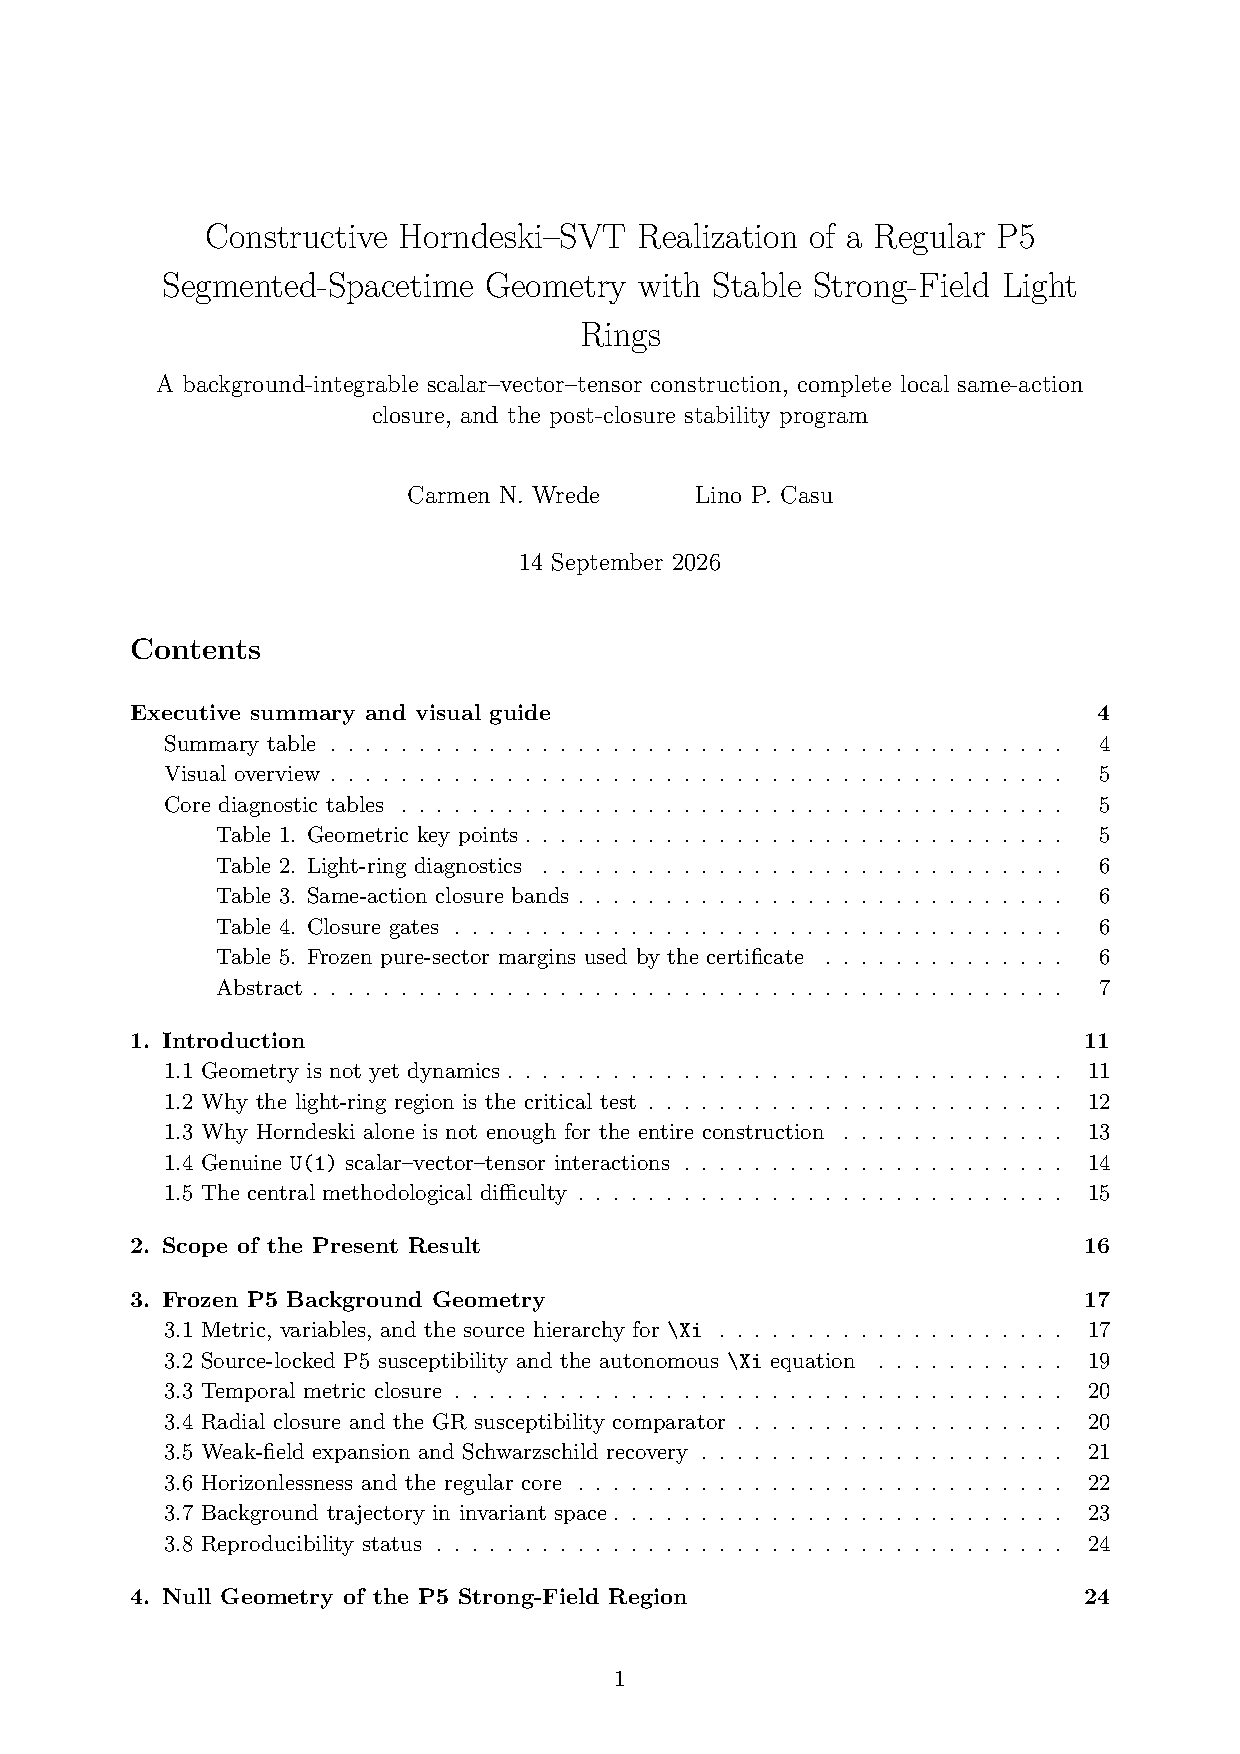
\includepdf[pages=-,pagecommand={}]{appendices/SSZ_P5_Horndeski_SVT_CLOSURE_COMPLETE_2026-09-14.pdf}
\section{Finite-$\ell$ technical memory, 2026-09-16}

\includepdf[pages=-,pagecommand={}]{appendices/SSZ_P5_HSVT_FINITE_L_TECHNICAL_MEMORY_2026-09-16.pdf}
\section{KRGM technical safety protocol, 2026-09-16}
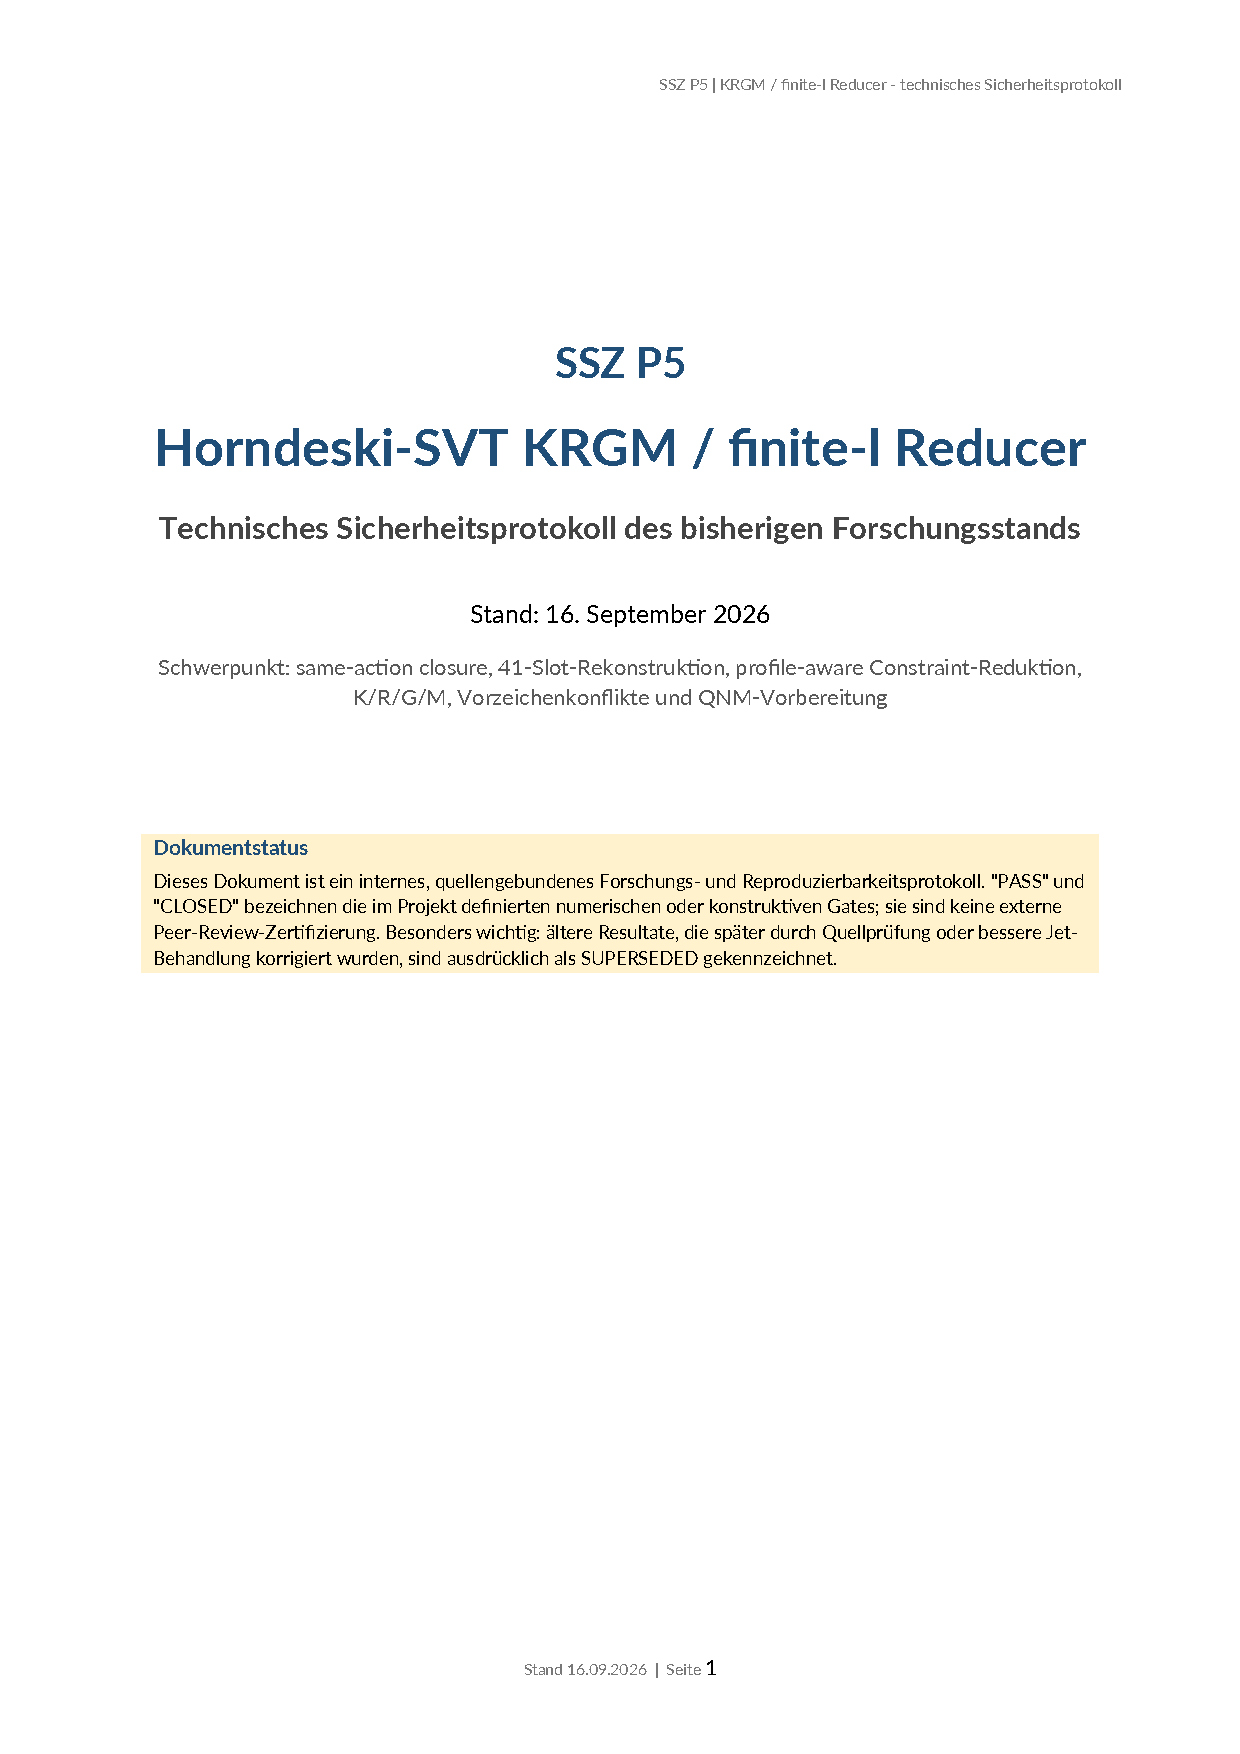
\includepdf[pages=-,pagecommand={}]{appendices/SSZ_P5_KRGM_TECHNISCHES_SICHERHEITSPROTOKOLL_2026-09-16.pdf}
\backmatter
\chapter{References}
\begin{thebibliography}{99}
\bibitem{KaseTsujikawa2023} R. Kase and S. Tsujikawa, ``Black hole perturbations in Maxwell-Horndeski theories,'' \emph{Phys. Rev. D} 107, 104045 (2023), arXiv:2301.10362.
\bibitem{ZhangKase2024} C. Zhang and R. Kase, ``Even-parity stability of hairy black holes in U(1) gauge-invariant scalar-vector-tensor theories,'' \emph{Phys. Rev. D} 110, 044047 (2024), arXiv:2404.11910.
\bibitem{Horndeski1974} G. W. Horndeski, ``Second-order scalar-tensor field equations in a four-dimensional space,'' \emph{Int. J. Theor. Phys.} 10, 363--384 (1974).
\bibitem{ReggeWheeler1957} T. Regge and J. A. Wheeler, ``Stability of a Schwarzschild singularity,'' \emph{Phys. Rev.} 108, 1063 (1957).
\bibitem{Zerilli1970} F. J. Zerilli, ``Effective potential for even-parity Regge-Wheeler gravitational perturbation equations,'' \emph{Phys. Rev. Lett.} 24, 737 (1970).
\end{thebibliography}
\end{document}
